
\section{Marco teórico}

En esta sección se muestran las bases sobre las que se sustenta el presente trabajo, se abordan los temas referentes al lenguaje de señas mexicano, así como el procesamiento involucrado en el reconocimiento de voz como es la adquisición de la señal de voz, su procesamiento y las técnicas a emplear para la detección de palabras, así como también la base de datos utilizada y las comunicaciones requeridas.

\subsection {Estructura básica de la oración}

Para definir las palabras y oraciones que serán empleadas para realizar la detección e interpretación a lenguaje de señas, se plantea el estudio de la estructura básica de la oración para el LSM ya que ésta presenta diferencias con la oración del idioma español que conocemos, esto con el fin de poder analizar las oraciones y determinar su equivalente en LSM.

Para empezar, debemos tomar en cuenta las particularidades que presentan las lenguas viso gestuales como el LSM, la tarea de describir la sintaxis que presentan las lenguas, ya sean orales o de señas, se debe reflexionar sobre dos nociones fundamentales: la proposición y la oración.

La proposición hace referencia a un proceso interno en el cual cada persona combina y manipula conceptos con el fin de comunicarse. Así, en una proposición se involucran una o dos entidades conceptuales con una relación, actividad o propiedad que les concierne. La oración es la expresión lingüística de una proposición.

Ahora bien, la oración básica o simple se caracteriza por ser la unidad sintáctica formada por la unión de un predicado y su sujeto.

El sujeto está constituido por una frase nominal que puede ser un nombre (con o sin determinantes, o con modificadores), un pronombre, o una oración, o bien puede estar ausente.

Por otra parte, el predicado es lo que se dice del sujeto, el verbo es el núcleo o palabra esencial de esta unidad sintáctica. En la LSM, así como en otras lenguas de señas, la clase de verbos (llanos y demostrativos) puede influir en el orden de constituyentes que presenta. Aunque de manera general se puede decir que en la LSM el orden de constituyentes que se observa en la mayoría de las construcciones gramaticales es Sujeto-Verbo-Objeto (SVO), se presentan las variaciones OSV, VOS, VSO, OVS y SOV, según el tipo de verbo que se utilice, así como por situaciones pragmáticas y semánticas. Por tanto, la LSM es una lengua cuyo orden responde no sólo a los principios que regulan las relaciones gramaticales sino además a aspectos semánticos y pragmáticos. \cite{Aldrete2008}

El LSM al igual que cualquier otro idioma se sustenta a base de reglas gramaticales para la estructuración de oraciones. La regla principal para el ordenamiento de frases es la siguiente.

\begin{centering}

Tiempo – Lugar – Sujeto – Objeto – Verbo

\end{centering}

\begin{itemize}

\item	Tiempo: establece el momento en que sucede la acción
\begin{itemize}
\item	Ejemplos: Antes, ahora, hoy, en el futuro, mientras, etc.
\end{itemize}
\item	Lugar: el sitio donde ocurre la acción
\begin{itemize}
\item	Ejemplos: Aquí, nombres de ciudades, países, etc.
\end{itemize}
\item	Objeto: Las personas o cosas que reciben la acción del sujeto
\begin{itemize}
\item	El objeto se indica antes del sujeto y debe ubicarse en un espacio.
\end{itemize}
\item	Sujeto: Las personas o coas que realizan la acción
\begin{itemize}
\item	El sujeto se indica inmediatamente antes de la acción que va a realizar y debe ubicarse en un espacio.
\end{itemize}
\item	Verbo: la acción
\begin{itemize}
\item	Ejemplos: Correr, hacer, platicar, seguir, etc.
\end{itemize}
\item	Preguntas: La palabra interrogante (cuándo, cómo, dónde) va al final, acompañada de la expresión facial.

\end{itemize}

Tomando en cuenta este último punto , si deseamos generalizar más la estructura obtenemos:

\begin{centering}
Tiempo – Lugar – Sujeto – Objeto – Verbo – Pregunta
\end{centering}

\subsection{¿Cómo formar oraciones?}

De acuerdo a la estructura anterior se darán unos ejemplos de cómo formar oraciones en LSM a partir de una en español.

\begin{itemize}

\item	Formar oraciones

\begin{itemize}
\item	Español: Fui rápido al mercado.
\begin{itemize}
\item	LSM: Pasado mercado yo ir rápido.
\end{itemize}
\item	Español: Yo jugué futbol el mes pasado en Cuernavaca.
\begin{itemize}
\item	LSM: Mes pasado Cuernavaca yo futbol jugar.
\end{itemize}
\item	Español: Próximo diciembre me iré de vacaciones a Acapulco.
\begin{itemize}
\item	Próximo diciembre Acapulco yo vacaciones ir.
\end{itemize}
\end{itemize}

\item	Oraciones interrogativas

\begin{itemize}
\item	Español: ¿Tienes hermanos?
\begin{itemize}
\item	LSM: ¿Tú hermanos tener cuántos?
\end{itemize}
\item	Español: ¿Qué quieres comer?
\begin{itemize}
\item	LSM: ¿Tú comer que significa?
\end{itemize}
\item	Español: ¿Cuáles son tus hermanos?
\begin{itemize}
\item	LSM: ¿Ellos hermanos tuyos cuáles?
\end{itemize}
\end{itemize}

\item	Oraciones y señas negativas

\begin{itemize}
\item	Español: Yo quiero un helado de chocolate, no de fresa.
\begin{itemize}
\item	LSM: Yo helado chocolate querer no fresa.
\end{itemize}
\item	Español: No me fui de vacaciones.
\begin{itemize}
\item	LSM: Agosto pasado yo vacaciones ir nada.
\end{itemize}
\item	Español: El pozole de la abuela no me gusta.
\begin{itemize}
\item	LSM: Yo pozole abuela no me gusta.
\end{itemize}
\end{itemize}

\end{itemize}

\subsection{Características de la señal de voz}

En esta sección se estudian las características de la señal de voz en el dominio del tiempo y la frecuencia, así como también se hace el análisis estadístico de la voz.

\subsubsection{Tiempo}

Básicamente de acuerdo al estado de la fuente de producción de voz podemos clasificar en tres estados a la señal de voz. Estos son: silencio (SL), en el que no hay voz; voz sorda (SR), en el que las cuerdas vocales no vibran, y voz sonora (SN) en el que las cuerdas vocales vibran dando lugar a una señal casi periódica. \cite{Mesa}

Como ejemplo en la Figura \ref{fig:sixOnda} se muestra la gráfica de la señal de voz correspondiente a la palabra six pronunciada por un hombre, el eje horizontal representa el tiempo en segundos y el eje vertical representa la amplitud de la señal. Inicialmente tenemos silencio hasta los 0.58 segundos, los siguientes 120 ms observamos que la señal es sorda correspondiente al fonema /s/ al cual le sigue un abrupto incremento de energía en un intervalo de 120 ms en el que la señal es sonora, perteneciente al fonema /I/, al que le sigue un silencio intrasilábico de 80 ms y finalmente otro intervalo de voz sorda, correspondientes a los fonemas /k/ y /s/, de alrededor de 230 ms seguidos de un silencio.

\begin{figure}[H]
	\centering
	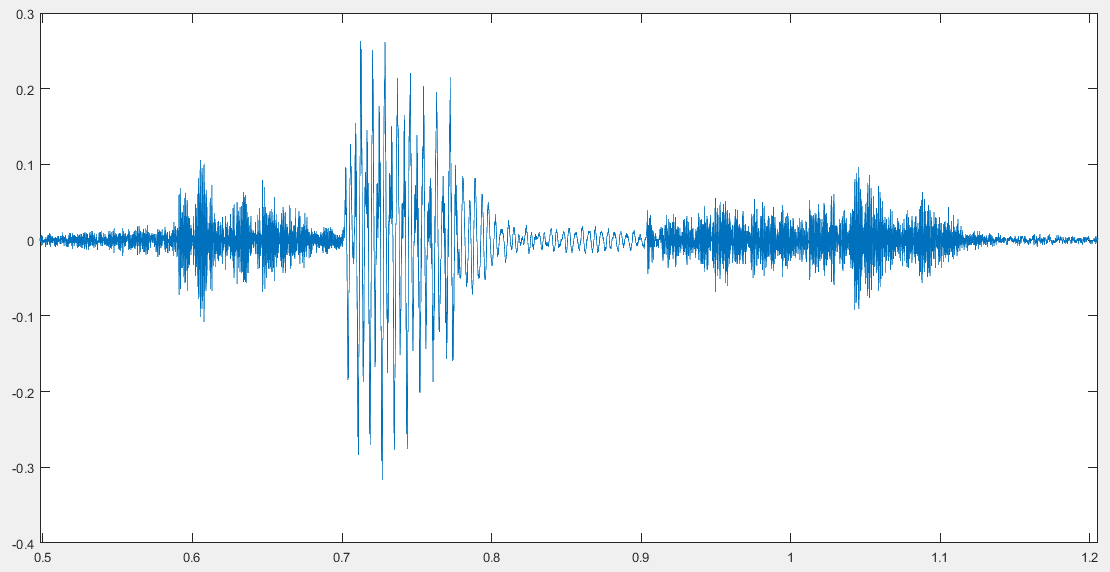
\includegraphics[width=1\linewidth]{figures/sixOnda}
	\caption{Forma de onda de la palabra ''six''}
	\label{fig:sixOnda}
\end{figure}

Una característica de la señal de voz que obtenemos en el dominio del tiempo es la energía de la señal, la cual es la suma del cuadrado del módulo de la señal o un intervalo de ésta, en el caso de la señal de voz es la suma del cuadrado de las amplitudes y queda definida de la siguiente forma:
		
\begin{equation}\label{eq:energia}
	E = \sum_{n=-\infty}^{\infty}{|x(n)|^2}
%	y = f \left[ \left( \sum_{i=1}^{N}\omega_i*x\left(n-i\right)\right)-b	\right]
\end{equation}		

Donde:
\\$E->$ energía de la señal.
\\$x->$ señal de voz.


La energía nos puede ser de utilidad para determinar si la señal de voz es sonora o sorda, de la Figura \ref{fig:sixOnda} podemos observar que la forma de onda del fonema /s/ tiene menor amplitud que la forma de onda correspondiente al fonema /I/, es evidente que, si tomamos un intervalo del mismo número de muestras para cada fonema, el valor de energía para esos intervalos será mayor para el fonema /I/ que representa una señal sonora. Esta técnica para determinar la clasificación de la señal de voz no es efectiva, ya que la señal sorda y el silencio se equiparán en amplitud lo cual causaría errores de clasificación.

El tono es otra característica de la voz, en \cite{MediaRadio} se dice que el tono es la impresión que nos produce la frecuencia de vibración a la que se manifiesta una determinada onda sonora, para el caso de la producción de la voz, la marca de tono (grave o agudo) viene dada por la cantidad de movimiento que se produce en las cuerdas vocales al emitirla, es decir, el número de vibraciones que en ellas tiene lugar. Dada la definición anterior, es posible determinar el tono de la señal de voz a partir de su representación en el tiempo.

\subsubsection{Frecuencia}

El concepto de formante es de gran importancia en cualquier tema relacionado con el análisis de la señal de voz, pues en ellos (en su distribución y estructura) está concentrada la mayor parte de la información psicoacústica transportada por la señal de voz que permite la comprensión del mensaje, éstos son picos en el espectro de voz consecuencia de las resonancias en el tracto vocal. \cite{Mesa}

Las frecuencias de resonancia son características esenciales de los formantes, las frecuencias de los tres primeros formantes pueden constituir un sistema de referencia absoluto para los sonidos vocálicos, en el que las distintas vocales quedan representadas de forma relativamente independiente del locutor.

El domino frecuencial nos permite conocer la estructura de los formantes, la representación espectral es una técnica que nos ayuda a conocer las características frecuenciales relevantes de la señal de voz. En la Figura \ref{fig:espectroSonora} (tomada de \cite{Mesa}) se aprecia el espectro correspondiente a una señal genérica de voz sonora, gracias a esta representación podemos observar características tales como los formantes o la frecuencia fundamental y sus armónicos. La frecuencia fundamental es la frecuencia de vibración de las cuerdas vocales. Para los hombres esta frecuencia está entre 100-125 Hz dependiendo de la edad y para las mujeres es de 200-250Hz. En la figura podemos distinguir tres formantes, F1, F2 y F3, así como la frecuencia fundamental, F0.

\begin{figure}[H]
	\centering
	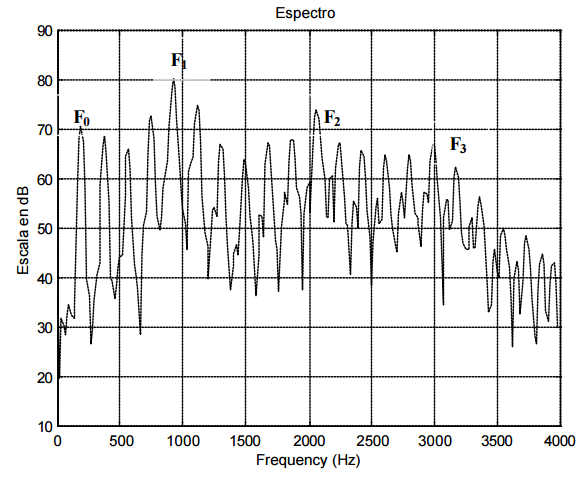
\includegraphics[width=0.8\linewidth]{figures/espectroSonora}
	\caption{Espectro de una señal sonora}
	\label{fig:espectroSonora}
\end{figure}

Una forma alterna de caracterizar la señal de voz y representar su información asociada es por medio de una representación conjunta de tiempo y frecuencia. El espectrograma es una representación tiempo frecuencia tridimensional en la que se muestra la intensidad de la voz y su evolución temporal en diferentes bandas frecuenciales.

En el espectrograma de banda ancha los sucesos temporales están resueltos con gran precisión mostrando, por ejemplo, barras verticales durante los intervalos sonoros asociados a los instantes de cierre glótico. La resolución frecuencial, a diferencia de la temporal, es pobre. Por el contrario, el espectrograma de banda estrecha tiene peor resolución temporal pero una mejor resolución frecuencial. En éste, los armónicos de la frecuencia fundamental están bien resueltos y definidos como líneas casi horizontales.

En la Figura \ref{fig:spectrogram} se muestra la forma de onda de la señal de voz, la magnitud del espectro en frecuencia y el espectrograma, en el cual se muestra la evolución de la potencia de los componentes frecuenciales a través del tiempo, podemos observar cómo aumenta la potencia de los componentes frecuenciales en el periodo de tiempo en que la amplitud de la forma de onda aumenta.

\begin{figure}[H]
	\centering
	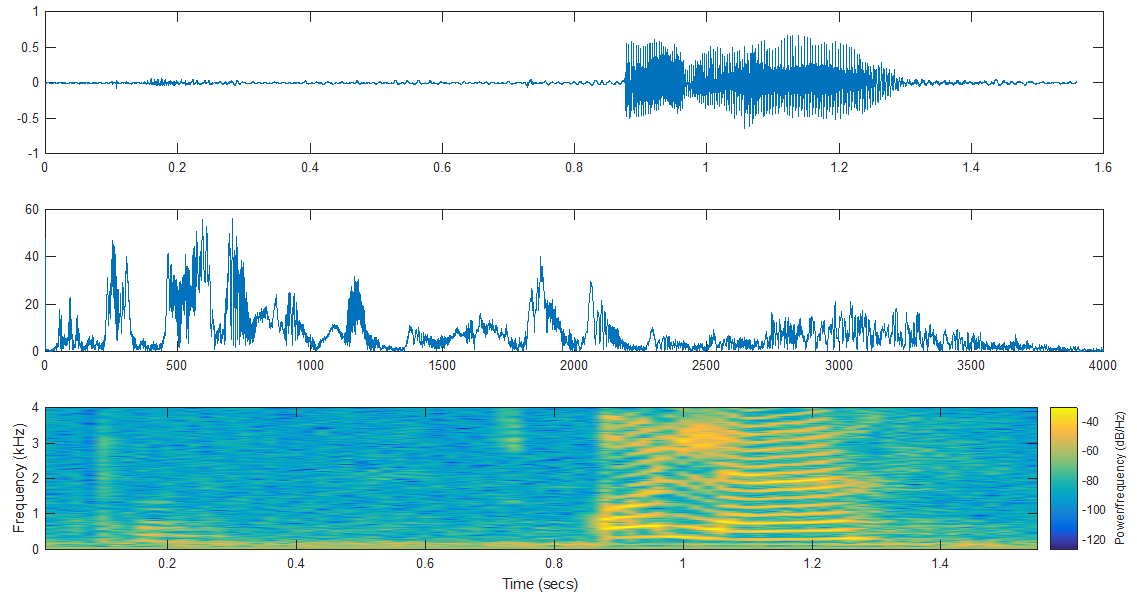
\includegraphics[width=1\linewidth]{figures/spectrogram}
	\caption{Espectrograma de la señal de voz}
	\label{fig:spectrogram}
\end{figure}

\subsubsection{Estadístico}

Algunos aspectos a estudiar sobre la naturaleza estadística de la voz son: función de densidad de probabilidad (FDP), estacionariedad y ergodicidad.

La FDP se puede estimar mediante un histograma de las amplitudes sobre un número suficientemente grande y representativo de muestras de señal. La estadística de la voz queda bien representada por una distribución laplaciana o, en mejor medida, por una distribución gamma.

En \cite{Mesa} se dice que en la mayoría de técnicas de extracción de características es conveniente hacer la suposición que la voz es un proceso estocástico ergódico y aunque resulta un modelo simplista, los resultados obtenidos en la práctica justifican su validez. Un ejemplo es que la autocorrelación de un proceso ergódico puede ser obtenida mediante la estimación de un promedio temporal conveniente. La estimación se tiene que hacer con un segmente suficientemente largo, aunque finito, de la señal. La validez del modelo ergódico está ligada a la suposición de la estacionariedad. La voz es un proceso estacionario o no según la longitud del intervalo de observación. La señal de voz es una señal de evolución lenta, cuando se observa en intervalos de tiempo suficientemente cortos (típicamente, entre 20 y 60 ms), sus características son prácticamente estacionarias. Se dice entonces que se trata de una señal casi estacionaria. Vista en intervalos largos (del orden de un cuarto de segundo o más) las características de la voz cambian para reflejar los diferentes sonidos que se están pronunciando, dando lugar a una señal no estacionaria. Por lo tanto, la validez de ergodicidad ha de entenderse en intervalos donde sea cierto que la señal es estacionaria.

En los sistemas de reconocimiento, la extracción de características se hace en tramas de la señal, de modo que podamos suponer estacionariedad y ergodicidad.

\subsection{Producción de la voz}

La voz humana es producida en la laringe, cuya parte esencial, la glotis, constituye el verdadero órgano de fonación humano. El aire procedente de los pulmones, es forzado durante la espiración a través de la glotis, haciendo vibrar los dos pares de cuerdas vocales, que se asemejan a dos lengüetas dobles membranáceas. Las cavidades de la cabeza, relacionadas con el sistema respiratorio y nasofaríngeo, actúan como resonadores. \cite{GrupodeAcustica2002}

El sistema vocal humano puede dividirse en tres partes:

\begin{itemize}
\item	Aparato respiratorio: donde se almacena y circula el aire. Nariz, pulmones, tráquea, diafragma.
\item	Aparato de fonación: donde el aire se convierte en sonido. Laringe y cuerdas vocales.
\item	Aparato resonador: donde el sonido adquiere sus cualidades de timbre que caracterizan cada voz. Cavidad bucal, faringe, paladar óseo, senos maxilares y frontales.
\end{itemize}

\begin{figure}[H]
	\centering
	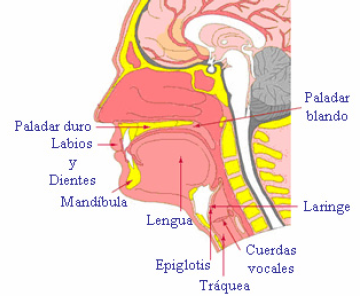
\includegraphics[width=0.6\linewidth]{figures/cavidadBucal}
	\caption{Cavidad bucal}
	\label{fig:cavidadBucal}
\end{figure}

De acuerdo al comportamiento de la cavidad bucal y la configuración de los órganos que participan en la generación de la voz, la señal generada puede clasificarse en dos tipos:

\begin{itemize}
\item	Señal sonora: se genera por la acción de las cuerdas vocales, las cuales se abren y cierran modificando el área de la tráquea y produciendo un tren de impulsos cuasi-periódicos. El período o frecuencia fundamental de este tren de impulsos se conoce con el nombre de pitch, y su valor está comprendido entre 50 y 400 Hz para los hombres y es superior en mujeres y niños. \cite{Alonso1999}
\item	Señal no sonora: el aire fluye libremente hasta alcanzar el tracto vocal al permanecer abiertas las cuerdas vocales, ésta presenta una estructura ruidosa tanto en el dominio del tiempo como en el de la frecuencia, no teniéndose formantes. Además, la energía de la señal es mucho menor que la de los sonidos sonoros. \cite{Alonso1999}
\end{itemize}

El tracto vocal actúa como una cavidad resonante para los sonidos sonoros, estando centradas las frecuencias de resonancia para la mayoría de la gente en 500 Hz y sus armónicos pares. Esta resonancia produce grandes picos en el espectro resultante, a los cuales se les llama formantes. Además, la señal tiene una naturaleza paso-baja y a partir de unos 4 KHz comienza a predominar el ruido.

Modelar el proceso de generación de la voz es útil en muchas aplicaciones, como la extracción de ciertos parámetros que permiten identificarla, ya que el tracto vocal se representa mediante un filtro que varía en el tiempo, dependiendo de la acción que se realiza al pronunciar una palabra. Si se obtienen dichos coeficientes, se tiene, por lo tanto, características de la señal de voz que nos permitirán identificarla.

En la Figura \ref{fig:modeloSimplificado} se muestra el modelo simplificado de la producción de la voz, el filtro que modela el tracto vocal tiene dos posibilidades de entrada, que dependerá de si la señal es sonora o no. Para señales sonoras, la excitación será un tren de impulsos de frecuencia controlada (pitch), mientras que para las señales no sonoras la excitación será ruido blanco. \cite{SalcedoCherubini2006}

\begin{figure}[H]
	\centering
	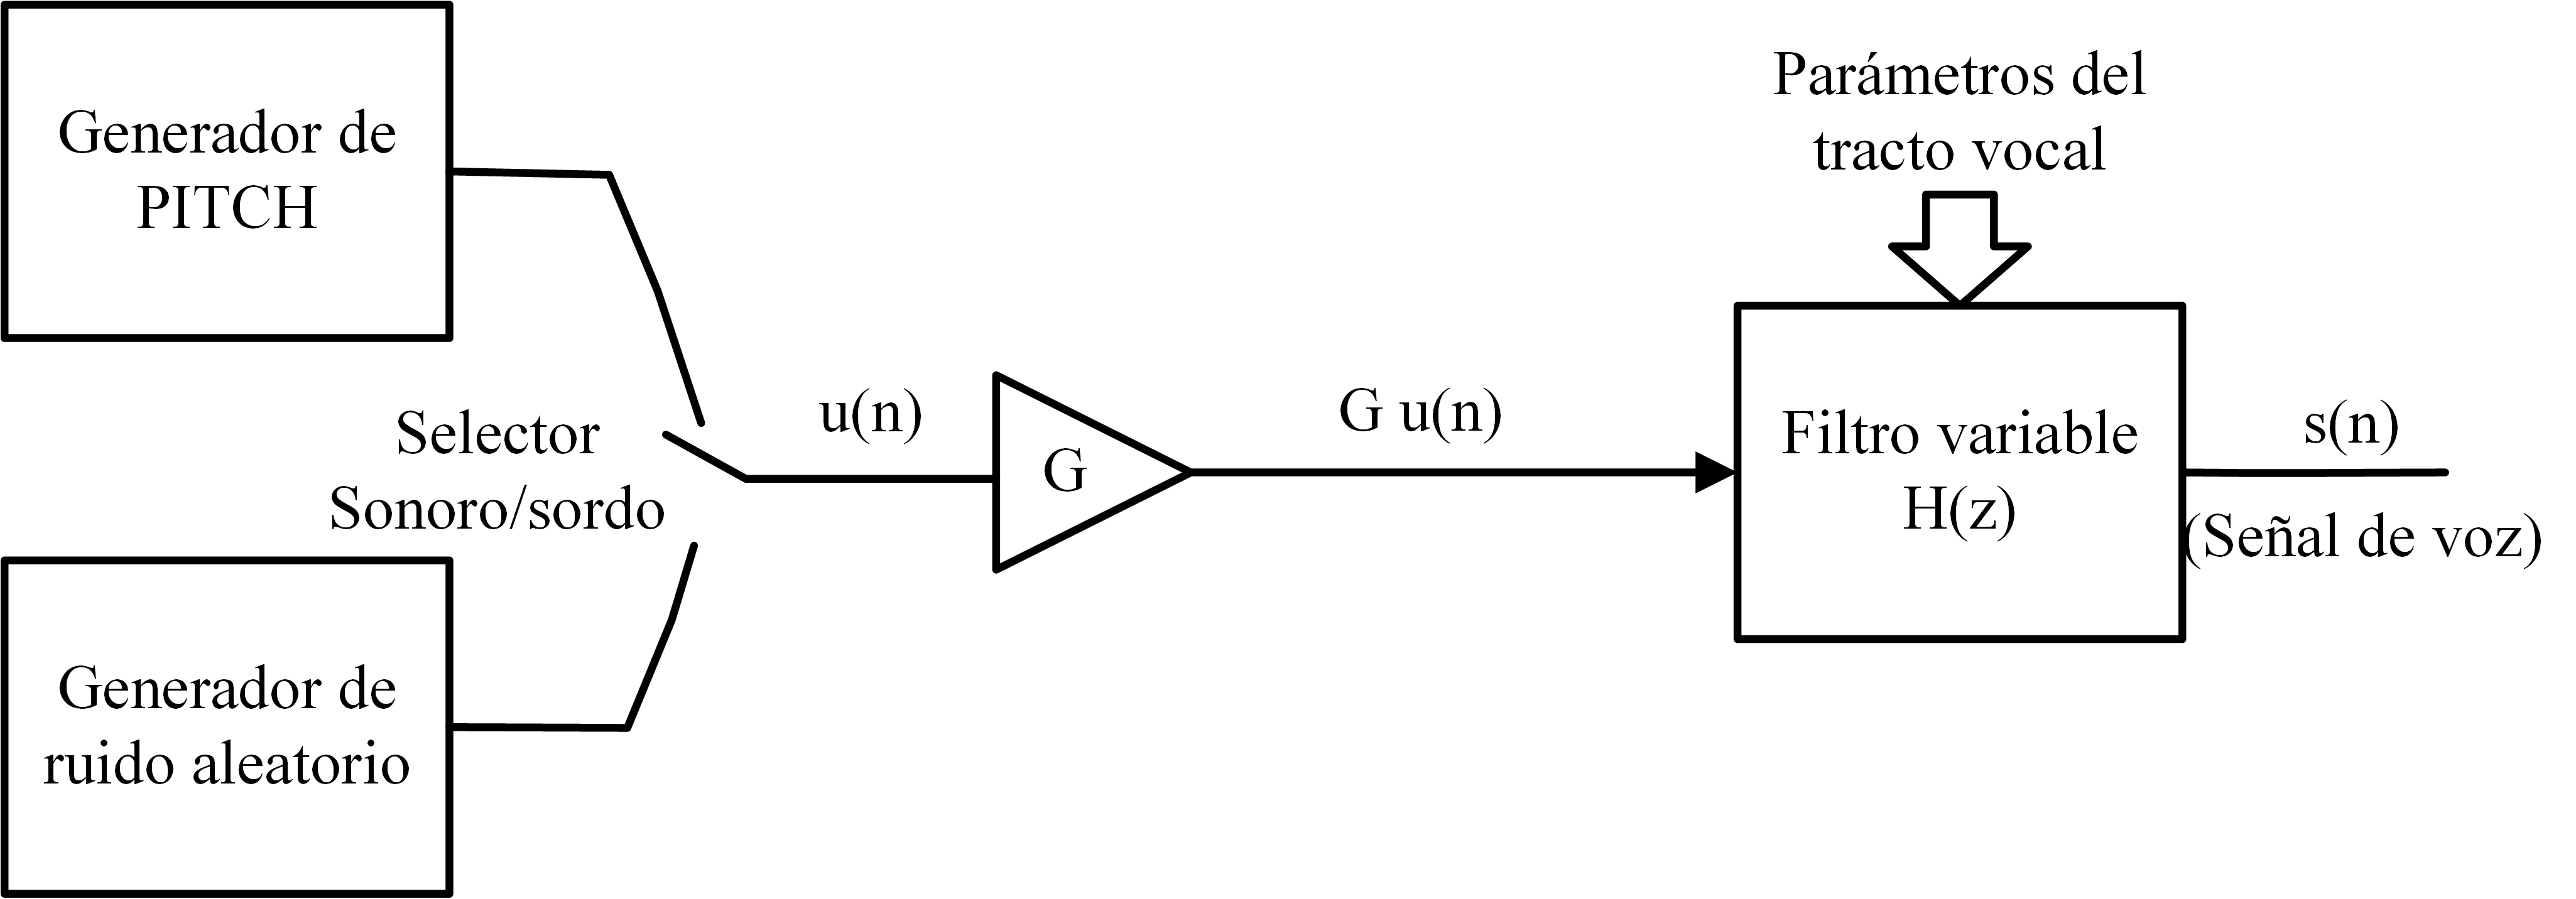
\includegraphics[width=0.8\linewidth]{figures/modeloSimplificado}
	\caption{Modelo Simplificado de la producción de la voz}
	\label{fig:modeloSimplificado}
\end{figure}

\subsection{Fonemas}

Los fonemas (sonido de la voz humana) son unidades teóricas básicas postuladas para estudiar el nivel fónico-fonológico de una lengua humana. Un fonema es cada una de las unidades segméntales postuladas para un sistema fonológico que dé cuenta de los sonidos de una lengua.

Los fonemas son la representación mental de un sonido, por ejemplo, si varias personas pronuncian la palabra tren, se notarán diferencias en la pronunciación más o menos marcadas, la t sonará más o menos enérgica, la r vibrará más o menos, estas variaciones serán notables, aunque la palabra sea pronunciada por el mismo hablante en situaciones diferentes. En la Figura \ref{fig:trenWord} se puede observar la pronunciación de la palabra Tren por tres personas diferentes, en este caso podemos observar las variaciones de amplitud de las palabras, y su duración. El sonido es la realización física de un fonema, en estos casos, podemos observar los diferentes sonidos que se generaron pero que corresponden al mismo fonema, por lo tanto, éstos son innumerables, tantos como hablantes y tantos como empleos le da cada hablante.

\begin{figure}[H]
	\centering
	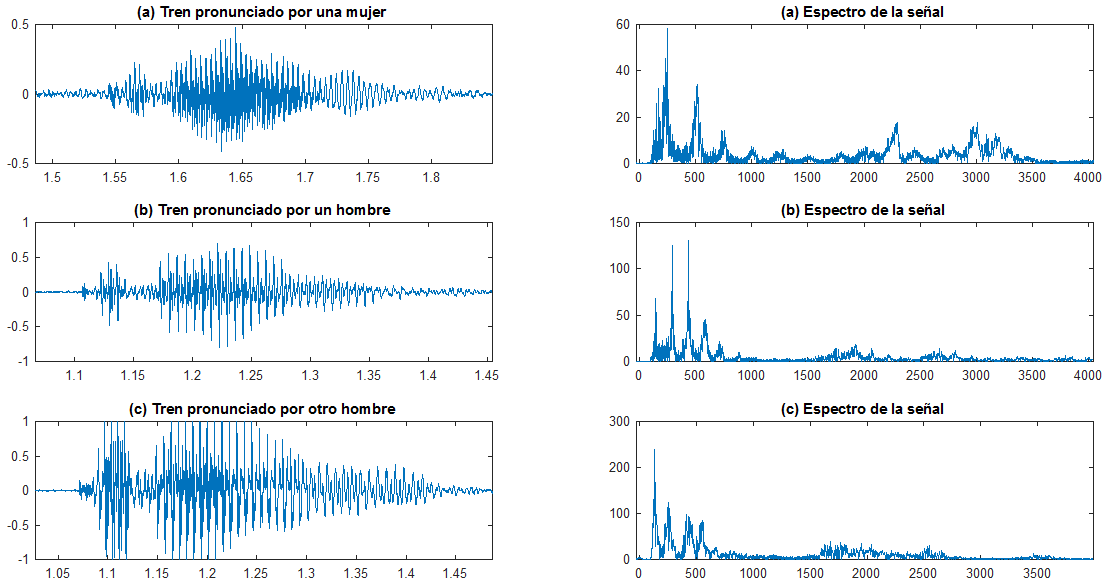
\includegraphics[width=1\linewidth]{figures/trenWord}
	\caption{Pronunciación de la palabra ''Tren''}
	\label{fig:trenWord}
\end{figure}

En la Figura \ref{fig:trenWord} podemos observar la diferencia de duración de pronunciación de palabras y la amplitud de la forma de onda que son las diferencias más visibles, por otro lado en el espectro de la señal se puede observar una gran diferencia entre el hombre y la mujer, ya que la mujer alcanza mayores frecuencias, incluso, la frecuencia fundamental está por encima de la de los hombres.

El sonido producido por las cuerdas vocales se le puede llamar un sonido “en bruto” ya que no ha sido modificado por la boca, este sonido en bruto al llegar a la boca es modificado para convertirse en sonido. Esta modificación es a lo que se le llama articulación. Articulación es la posición que adoptan los órganos de la boca en el momento de producir un sonido. Los órganos articuladores se clasifican en dos tipos:

\begin{itemize}
\item	Activos: éstos son el labio, la lengua, los dientes inferiores, velo del paladar. 
\item	Pasivos: dientes superiores, alvéolos\footnote{Los alvéolos son los hoyos donde están encajados los dientes, pero en fonética dicha palabra se refiere únicamente a las encías superiores, la zona en la que se apoya la lengua al pronunciar la n.}  superiores y paladar.
\end{itemize}

\subsubsection{Fonemas vocálicos}

Cuando articulamos los sonidos vocálicos, el aire no encuentra obstáculos en su salida desde los pulmones al exterior. Para clasificar estos fonemas, se tienen en cuenta los siguientes factores:

\begin{itemize}
\item	La localización o punto de articulación: Se refiere a la parte de la boca donde se articulan, pueden ser anteriores (/e/, /i/), medio o central (/a/) o posteriores (/o/, /u/).
\item	La abertura o modo de articulación: Se refiere a la abertura de la boca al pronunciarlos. Pueden ser de abertura máxima o abierto (/a/), de abertura media o semiabiertos (/e/, /o/) y de abertura mínima o cerrados (/i/, /u/). \cite{SantosPosada2004}
\end{itemize}

En la Figura \ref{fig:trianguloArticulatorio} se observa el triángulo articulatorio de las vocales o triángulo de Hellwag, el cual nos describe la localización y la abertura para cada fonema vocálico.

\begin{figure}[H]
	\centering
	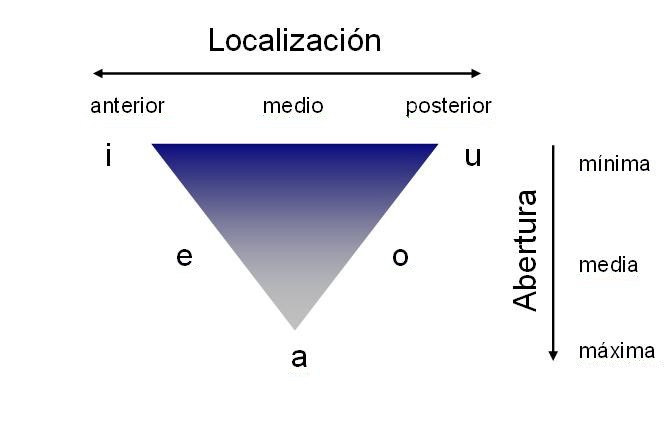
\includegraphics[width=0.8\linewidth]{figures/trianguloArticulatorio}
	\caption{Triángulo articulatorio de las vocales}
	\label{fig:trianguloArticulatorio}
\end{figure}

\subsubsection{Fonemas consonánticos}

En la articulación de los sonidos consonánticos siempre hay un obstáculo que impide salir el aire desde los pulmones al exterior. Según las circunstancias que rodean esta salida de aire, existen ciertos factores a tomar en cuenta a la hora de clasificarlos.

\begin{itemize}
\item	Zona o punto de articulación: Es el lugar donde toman contacto los órganos que intervienen en la producción del sonido.
\begin{itemize}
\item	Bilabial: Los dos labios.
\item	Labiodental: Labio inferior y dientes superiores.
\item	Interdental: Lengua entre los dientes.
\item	Dental: Lengua detrás de los dientes superiores.
\item	Alveolar: Lengua sobre la raíz de los dientes superiores.
\item	Palatal: Lengua y paladar.
\item	Velar: Lengua y velo del paladar.
\end{itemize}
\item	Modo de articulación: Es la postura que adoptan los órganos que producen los sonidos.
\begin{itemize}
\item	Oclusivo: Cierre total y momentáneo del paso del aire.
\item	Fricativo: Estrechamiento por donde pasa el aire rozando.
\item	Africado: Se produce una oclusión y después una fricación.
\item	Lateral: El aire pasa rozando los lados de la cavidad bucal.
\item	Vibrante: El aire hace vibrar la punta de la lengua al pasar.
\end{itemize}
\item	Actividad de las cuerdas vocales: Cuando producimos sonidos, las cuerdas vocales pueden vibrar o no vibrar.
\begin{itemize}
\item	Sordo: No vibran las cuerdas vocales.
\item	Sonoro: Vibran las cuerdas vocales.
\end{itemize}
\item	Actividad de la cavidad nasal: Si al producir sonidos, parte del aire pasa por la cavidad nasal, los sonidos se llaman nasales.
\begin{itemize}
\item	Nasal: Parte del aire pasa por la cavidad nasal.
\item	Oral: Todo el aire pasa por la boca.
\end{itemize}
\end{itemize}

En la Figura \ref{fig:fonemasConsonantes} se presentan los fonemas consonantes de acuerdo a los factores y rasgos mencionados anteriormente.

\begin{figure}[H]
	\centering
	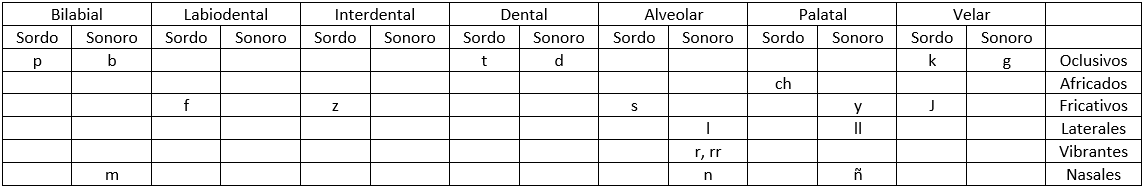
\includegraphics[width=1\linewidth]{figures/fonemasConsonantes}
	\caption{Cuadro de los fonemas consonantes}
	\label{fig:fonemasConsonantes}
\end{figure}

% Please add the following required packages to your document preamble:
% \usepackage{booktabs}
%\begin{table}[H]
%\centering
%\caption{My caption}
%\label{tbl:fonemas}
%\begin{tabular}{|p{0.8cm} |p{0.8cm} |p{0.8cm} |p{0.8cm} |p{0.8cm} |p{0.8cm} |p{0.8cm} |p{0.8cm} |p{0.8cm} |p{0.8cm} |p{0.8cm} |p{0.8cm} |p{0.8cm} |p{0.8cm} |p{0.8cm}|  }
%\toprule
%\multicolumn{2}{|c|}{Bilabial} & \multicolumn{2}{c|}{Labiodental} & \multicolumn{2}{c|}{Interdental} & \multicolumn{2}{c|}{Dental} & \multicolumn{2}{c|}{Alveolar} & \multicolumn{2}{c|}{Palatal} & \multicolumn{2}{c|}{Velar} &            \\ \midrule
%Sordo         & Sonoro         & Sordo          & Sonoro          & Sordo          & Sonoro          & Sordo        & Sonoro       & Sordo         & Sonoro        & Sordo        & Sonoro        & Sordo       & Sonoro       &            \\ \midrule
%p             & b              &                &                 &                &                 & t            & d            &               &               &              &               & k           & g            & Oclusivos  \\ \midrule
%              &                &                &                 &                &                 &              &              &               &               & ch           &               &             &              & Africados  \\ \midrule
%              &                & f              &                 & z              &                 &              &              & s             &               &              & y             & j           &              & Fricativos \\ \midrule
%              &                &                &                 &                &                 &              &              &               & l             &              & ll            &             &              & Laterales  \\ \midrule
%              &                &                &                 &                &                 &              &              &               & r, rr         &              &               &             &              & Vibrantes  \\ \midrule
%              & m              &                &                 &                &                 &              &              &               & n             &              & ñ             &             &              & Nasales    \\ \bottomrule
%\end{tabular}
%\end{table}

\subsection{Digitalización de la señal de voz}

La parte inicial de todo subsistema de preproceso de la señal de voz está constituida por:
\begin{itemize}
\item	Un micrófono, que convierte la onda sonora de presión en una señal eléctrica.
\item	Un amplificador, que amplifica hasta niveles manejables la débil señal que proporciona el micrófono.
\end{itemize}


\subsubsection{Muestreo y cuantificación}

A partir de la señal eléctrica que produce el amplificador se termina por digitalizar la señal de voz por un convertidor analógico/digital, éste, básicamente debe realizar dos tareas:

\begin{itemize}
\item	Muestrear la señal analógica; es decir, medir la amplitud de dicha señal cada cierto intervalo de tiempo.
\item	Cuantificar la señal muestreada; es decir, codificar numéricamente el resultado de cada una de las medidas.
\end{itemize}
De esta manera, una función continua del tiempo quedará representada por una serie discreta de valores numéricos.

\subsubsection*{Muestreo}

Una señal muestreada a intervalos de tiempo $T, s_M (t)$, puede definirse como el producto de la señal continua $s(t)$ y una función de Dirac (Figura \ref{fig:muestreoDelta}):

\begin{equation}\label{eq:muestreo}
	s_M(t)=s(t) \cdot \sum_{k=-\infty}^{\infty}\delta(t-KT)=\sum_{k=-\infty}^{\infty}s(kT)\delta(t-KT)
%	y = f \left[ \left( \sum_{i=1}^{N}\omega_i*x\left(n-i\right)\right)-b	\right]
\end{equation}

Donde:
\\$s_M->$ señal muestreada.
\\$s->$ señal a muestrear.		

\begin{figure}[H]
	\centering
	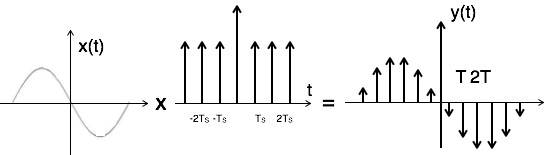
\includegraphics[width=0.6\linewidth]{figures/muestreoDelta}
	\caption{Muestreo de una señal}
	\label{fig:muestreoDelta}
\end{figure}

De donde es inmediato demostrar que la expresión del espectro $S_M (j\omega)$ de la señal muestreada en función de la señal sin muestrear $S(j\omega)$, adopta la forma:

\begin{equation}\label{eq:muestreoEspectro}
	S_M(j\omega)=\frac{1}{T}\sum_{k=-\infty}^{\infty}S[j(\omega+k\omega_0)] ;	 \omega_0=\frac{2\pi}{T}
%	y = f \left[ \left( \sum_{i=1}^{N}\omega_i*x\left(n-i\right)\right)-b	\right]
\end{equation}	

Expresión que representa la superposición del espectro de s(t) con las sucesivas versiones del mismo desplazadas en el eje de la frecuencia con periodicidad $\frac{1}{T}$.

De la Figura \ref{fig:aliasing} se observa que, si el ancho de banda de la señal a muestrear es excesivo con relación a la frecuencia de muestreo, se producirá un solapamiento irreversible de los espectros sucesivos, haciendo imposible la reconstrucción de la señal original. Este solapamiento (aliasing) ocurre siempre que la máxima frecuencia (Fb) del espectro de la señal a muestrear sea superior a la mitad de la frecuencia de muestreo (Fm) (frecuencia de Nyquist).

\begin{figure}[H]
	\centering
	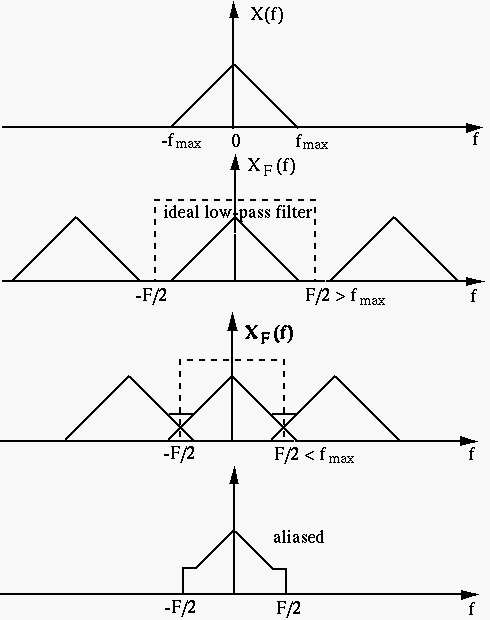
\includegraphics[scale = 0.6]{figures/aliasing}
	\caption{Efecto de solapamiento ''aliasing''}
	\label{fig:aliasing}
\end{figure}

Antes de muestrear una señal será pues necesario limitar la frecuencia máxima de ésta a la mitad de la de muestreo, lo que se puede conseguir mediante un filtro analógico de paso bajo previo al convertidor A/D, cuya frecuencia de corte sea la de Nyquist como máximo. La anchura de banda de la señal resultante deberá preservar la información relevante necesaria para una adecuada descripción de los objetos acústicos a tratar. \cite{Casacuberta1987}

\subsubsection*{Cuantificación}

El cuantificador es un sistema no lineal cuyo propósito es transformar la muestra de entrada $x[n]$ en un valor de un conjunto finito de valores preestablecidos. Representada como

\begin{equation}\label{eq:cuantificador}
	\hat{x}[n]=Q(x[n])
%	y = f \left[ \left( \sum_{i=1}^{N}\omega_i*x\left(n-i\right)\right)-b	\right]
\end{equation}	

Donde $\hat{x}[n]$ es la muestra cuantificada.

Los cuantificadores se pueden definir con niveles de cuantificación uniformes o no uniformes. La Figura \ref{fig:cuantificadorTipico} muestra la característica de transferencia de un cuantificador uniforme en el que los valores de las muestras se redondean hasta el nivel de cuantificación más próximo.

\begin{figure}[H]
	\centering
	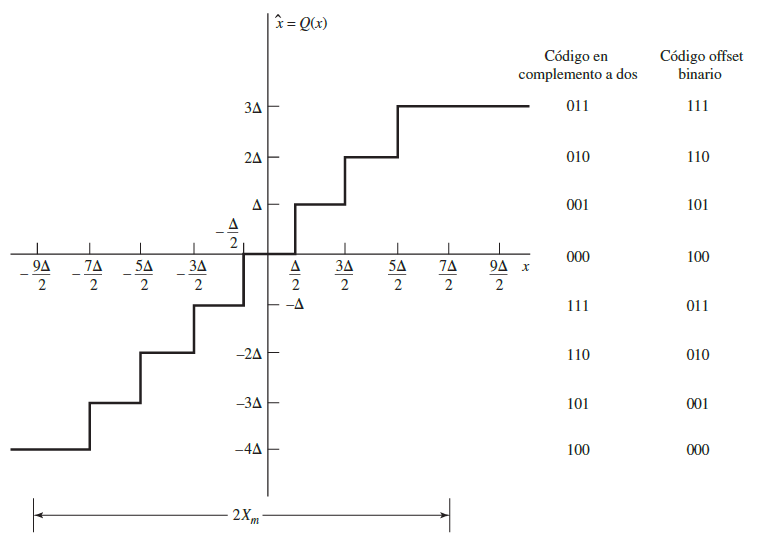
\includegraphics[scale = 0.6]{figures/cuantificadorTipico}
	\caption{Cuantificador típico para conversión A/D. (Tomado de \cite{Oppenheim2011})}
	\label{fig:cuantificadorTipico}
\end{figure}

\subsection{Métodos en el dominio del tiempo para el procesamiento del habla}

El objetivo en el procesamiento del habla es obtener la representación más útil de la información que lleva la señal de voz. La precisión requerida de esta representación está dada por información particular de la señal de voz que va a ser preservada o, en ciertos casos, resaltarla. Por ejemplo, el propósito del procesamiento digital puede ser para facilitar la identificación de la forma de onda correspondiente a voz o no. En una aplicación similar pero más complejo, queremos clasificar la señal de voz en 3 tipos, voz sonora, voz no sonora y silencio o ruido de fondo.

En esta sección se presentan técnicas de procesamiento en el dominio del tiempo.

\subsubsection{Procesamiento del habla dependiente del tiempo}

En la Figura \ref{fig:vozTipica} se muestra la representación típica de la señal de voz en la cual se aprecia que las propiedades de la voz cambian en el tiempo. Por ejemplo, la excitación cambia entre la señal sonora y la no sonora, hay variaciones significantes en la amplitud pico de la señal y hay una variación considerable de la frecuencia fundamental en las regiones de señal sonora.

\begin{figure}[H]
	\centering
	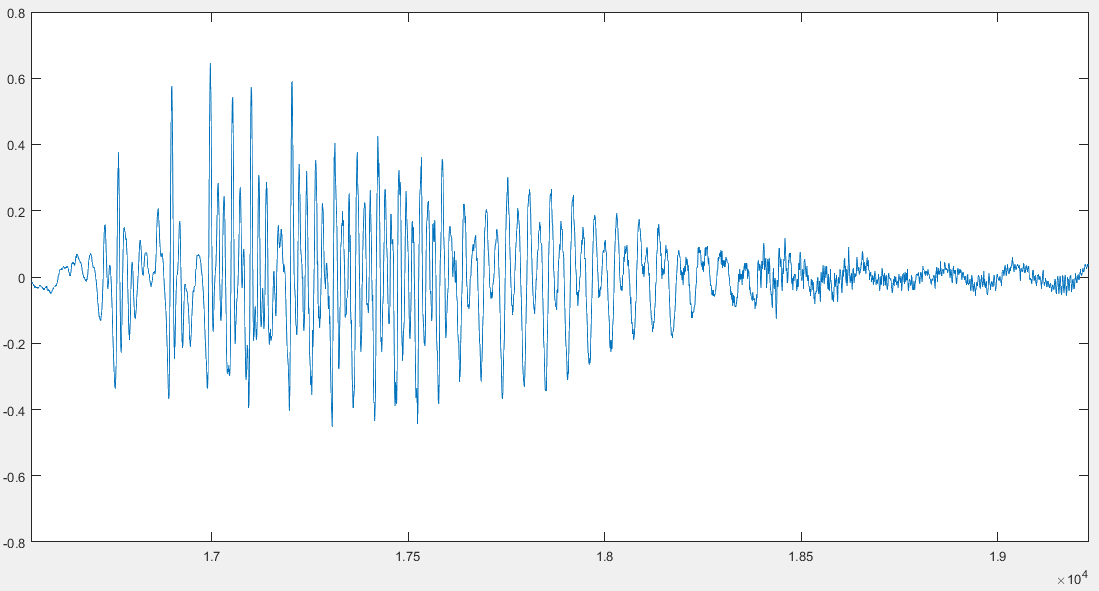
\includegraphics[width=1\linewidth]{figures/vozTipica}
	\caption{Señal de voz}
	\label{fig:vozTipica}
\end{figure}

Estas variaciones son evidentes en una gráfica de la forma de onda en el dominio del tiempo, por lo cual, las técnicas de procesamiento deben ser capaces de ofrecernos representaciones útiles de las características de la señal como la intensidad, modo de excitación, tono, y posiblemente parámetros del tracto vocal como frecuencias formantes.

La suposición en muchos esquemas de procesamiento del habla es que las propiedades de la señal cambian relativamente lento con el tiempo. Esta suposición deja una variedad de métodos de procesamiento en tiempo corto en donde segmentos cortos de la señal de voz son aislados y procesados como si fueran segmentos cortos de un sonido prolongado con propiedades fijas. El resultado del procesamiento de cada segmento puede ser tanto un número, o un conjunto de números. Por lo tanto, tal procesamiento produce una nueva secuencia dependiente del tiempo que puede servir como una representación de la señal de voz.

La mayoría de las técnicas de procesamiento en corto tiempo, así como la representación de Fourier en tiempo corto, pueden ser representadas matemáticamente con la ecuación \ref{eq:windowing}

\begin{equation}\label{eq:windowing}
	Q_n=\sum_{m=-\infty}^{\infty}{T[x(m)]w(n-m)}
%	y = f \left[ \left( \sum_{i=1}^{N}\omega_i*x\left(n-i\right)\right)-b	\right]
\end{equation}

La señal de voz es sujeta a una transformación, T[ ], que puede ser linear o no linear. La secuencia resultante es multiplicada por una ventana ubicada en un momento correspondiente al índice de muestra m. 

Una de las características de la seña de voz es la energía, ésta en una señal de tiempo se define como:

\begin{equation}\label{eq:windowing}
	E=\sum_{m=-\infty}^{\infty}{x^2(m)}
\end{equation}

Donde:
\\$E->$ energía de la señal.
\\$x->$ señal de tiempo.

Tal cantidad tiene poco significado o utilidad para el habla ya que da poca información acerca de las propiedades dependientes del tiempo de la señal de voz. La definición de la energía en poco tiempo es:

\begin{equation}\label{eq:windowing}
	E_n=\sum_{m=n-N+1}^{n}{x^2(m)}
\end{equation}

\subsubsection{Energía de corta duración y media de magnitud}

Se ha observado que la amplitud de la señal de voz varía con el tiempo. En particular, la amplitud de los segmentos de la señal no sonora es generalmente menor que la amplitud de los segmentos de señal sonora. La energía de corta duración de la señal de voz ofrece una representación conveniente que refleja estas variaciones de amplitud. En general, se puede definir la energía de corta duración como

\begin{equation}\label{eq:windowing}
	E_n=\sum_{m=-\infty}^{\infty}{[x(m)w(n-m)]^2}
\end{equation}

Donde:
\\$E_n->$ energía de corta duración.
\\$x->$ señal de voz.
\\$w->$ ventana aplicada.

$E_n$ proporciona una base para distinguir los segmentos de voz sonora delos segmentos de voz no sonora. Como se muestran en la Figura \ref{fig:energiaRectangular} y Figura \ref{fig:energiaHamming}, los valores de$ E_n$ para los segmentos de voz no sonora son menores que para los de la voz sonora. La función de energía también se puede usar para localizar aproximadamente el tiempo en el cual la voz sonora se convierte en voz no sonora, y viceversa, y, para una señal de muy alta calidad (alta relación señal a ruido), la energía puede ser usada para distinguir la voz del silencio.

\begin{figure}[H]
	\centering
	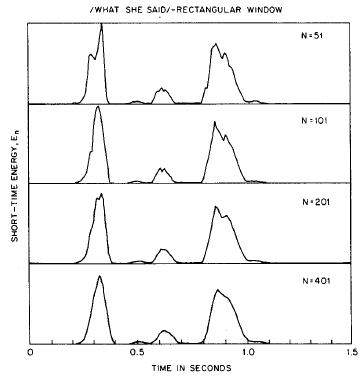
\includegraphics[width=0.5\linewidth]{figures/energiaRectangular}
	\caption{Energía en tiempo corto con ventana rectangular de varios tamaños}
	\label{fig:energiaRectangular}
\end{figure}

\begin{figure}[H]
	\centering
	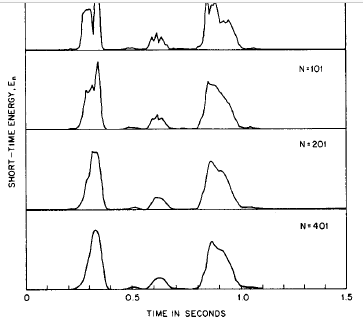
\includegraphics[width=0.5\linewidth]{figures/energiaHamming}
	\caption{Función de energía en periodo corto con ventana de Hamming en varios tamaños}
	\label{fig:energiaHamming}
\end{figure}

El promedio de la magnitud también es usado en el procesamiento de voz y aplicado a las señales de voz, la función de magnitud está dada por:

\begin{equation}\label{eq:promedio}
	M_n=\sum_{m=-\infty}^{\infty}{|x(m)|w(n-m)}
\end{equation}

Donde:
\\$M_n->$ promedio de magnitud.

Donde la suma ponderada de los valores absolutos de la señal es calculada en vez de la suma de cuadrados. La Figura \ref{fig:energiaFiltro} muestra cómo puede ser implementado como un filtro lineal sobre el absoluto de la señal. Este método logra simplificar aritméticamente la operación eliminando la operación de elevación al cuadrado.

\begin{figure}[H]
	\centering
	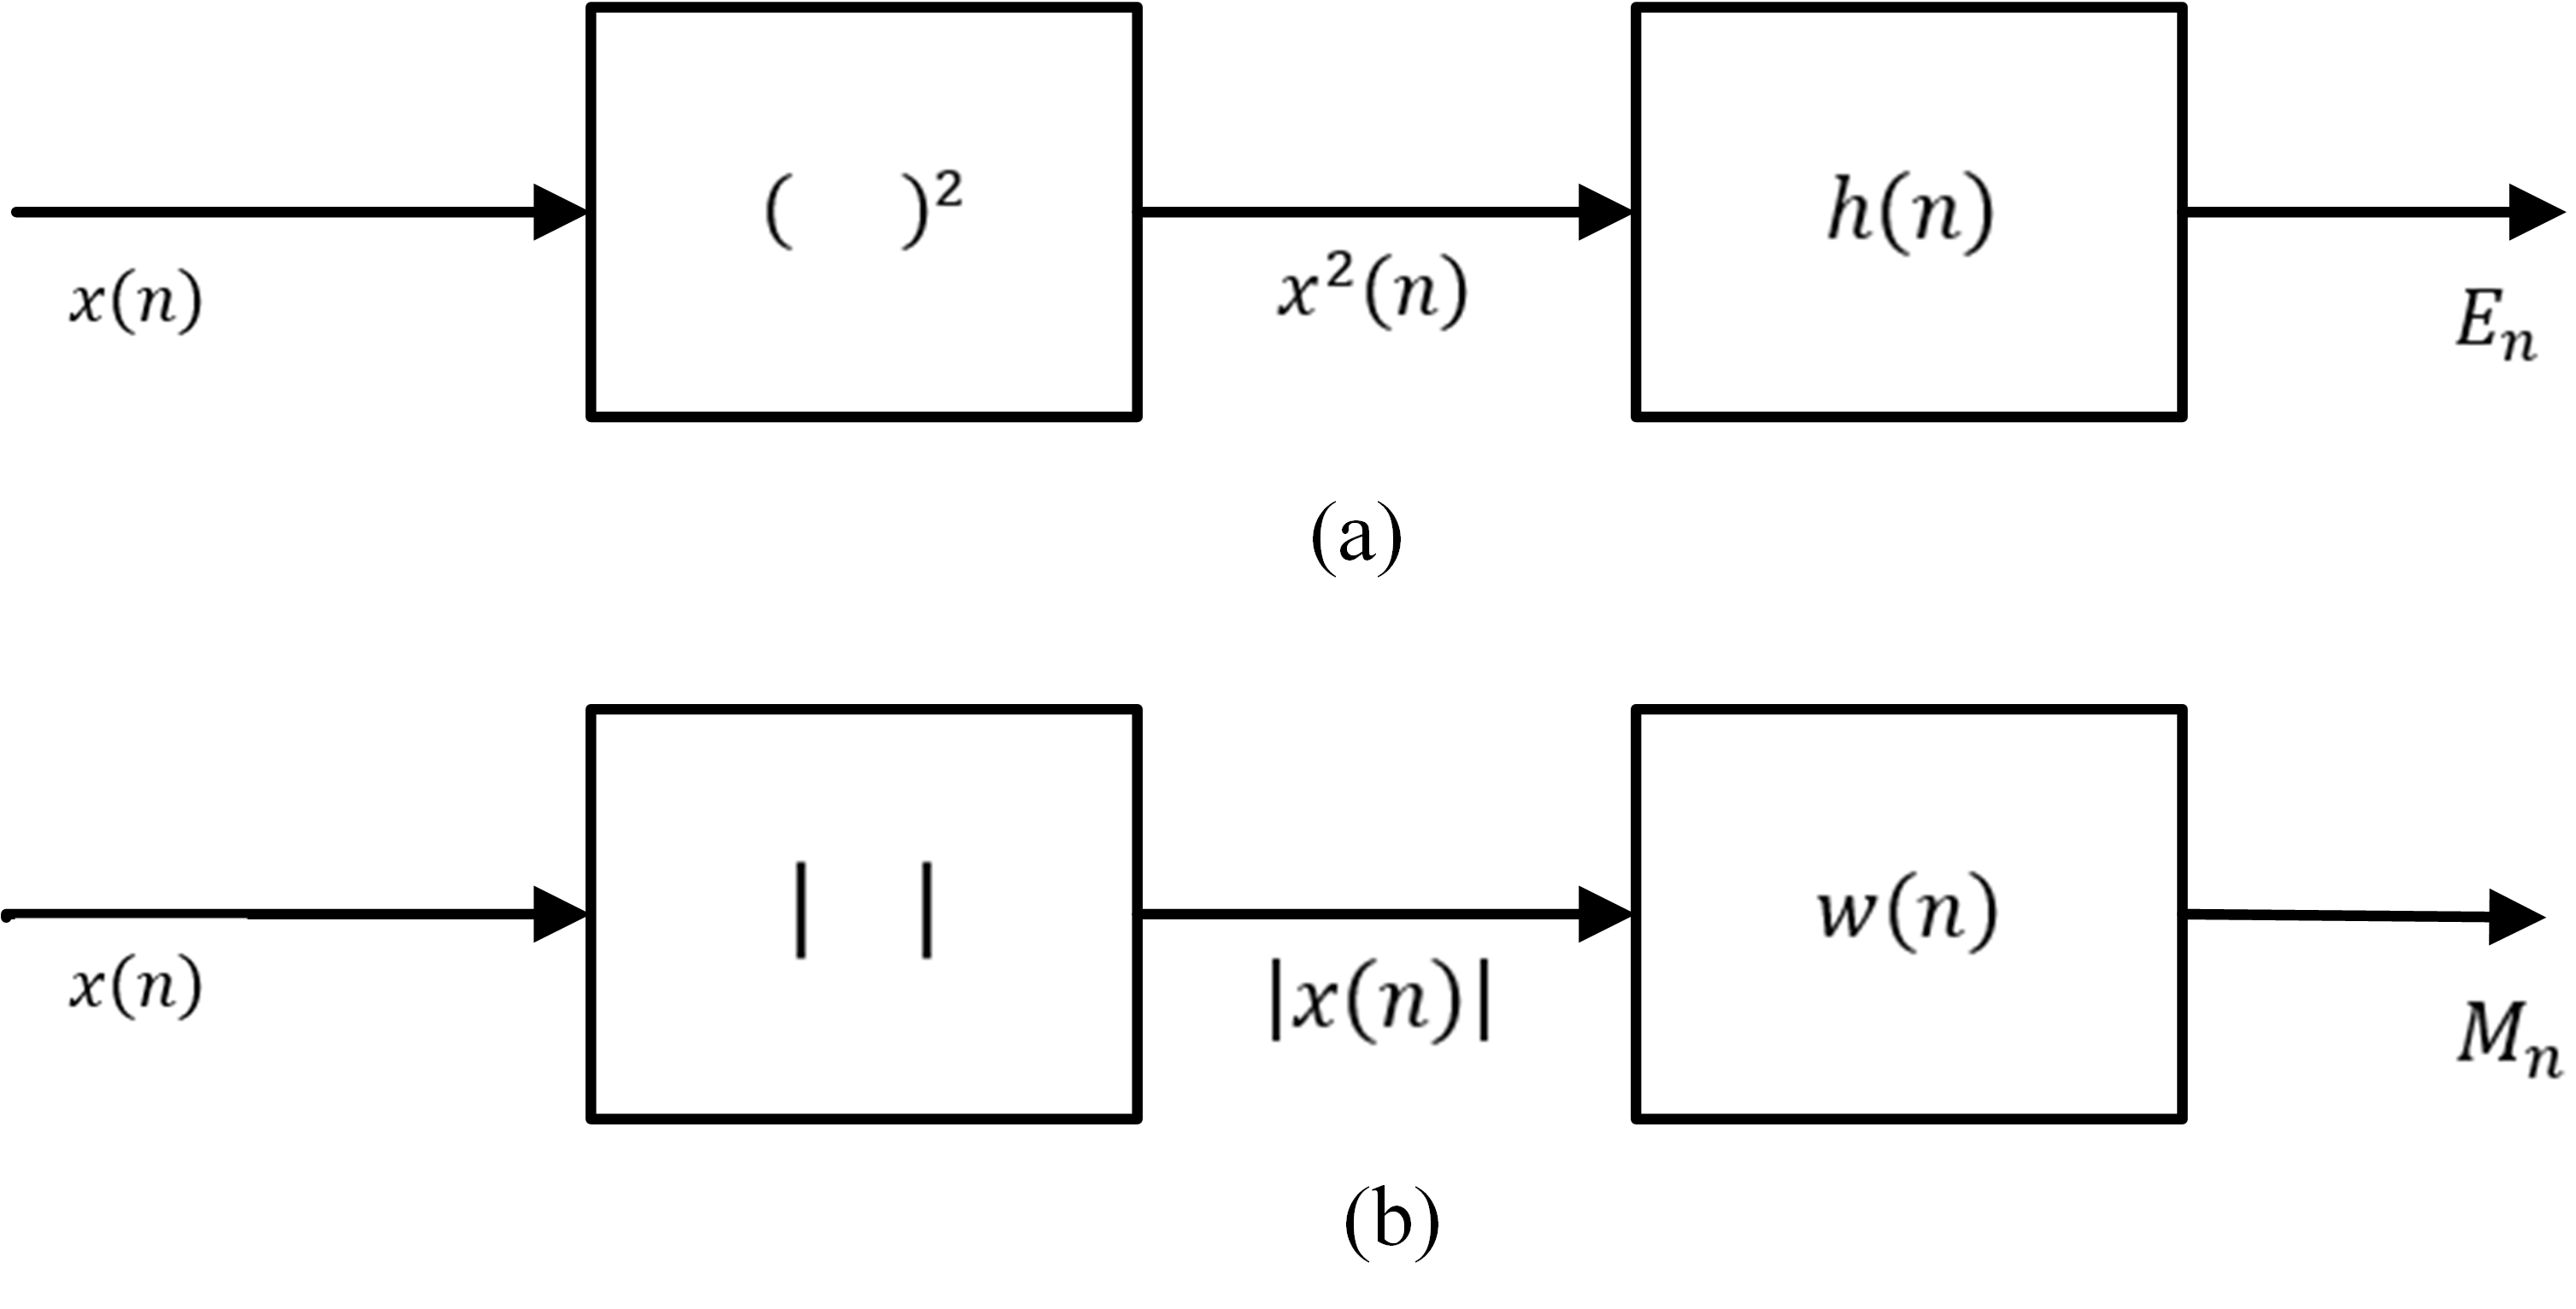
\includegraphics[width=0.5\linewidth]{figures/energiaFiltro}
	\caption{(a) Implementación del cálculo de la energía mediante un filtro. (b) implementación del cálculo de la magnitud promedio mediante un filtro}
	\label{fig:energiaFiltro}
\end{figure}

En la Figura \ref{fig:promedioRectangular} y Figura \ref{fig:promedioHamming} muestran las gráficas del promedio de la magnitud, en comparación con los resultados por el método de la energía se pueden observar diferencias muy notables en las regiones no sonoras. Para el promedio de la magnitud, el rango dinámico es aproximadamente la raíz cuadrada que el rango dinámico para el cálculo por energía. Por lo tanto, las diferencias de nivel entre las regiones sonoras y no sonoras no son tan notables como para el cálculo de energía en tiempo corto.

\begin{figure}[H]
	\centering
	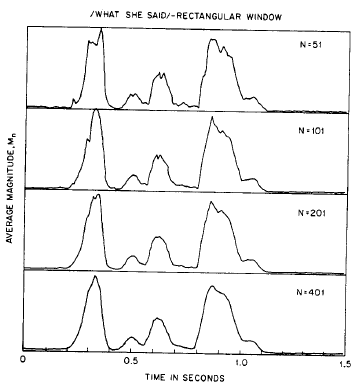
\includegraphics[width=0.5\linewidth]{figures/promedioRectangular}
	\caption{Promedio de magnitud con ventana rectangular}
	\label{fig:promedioRectangular}
\end{figure}

\begin{figure}[H]
	\centering
	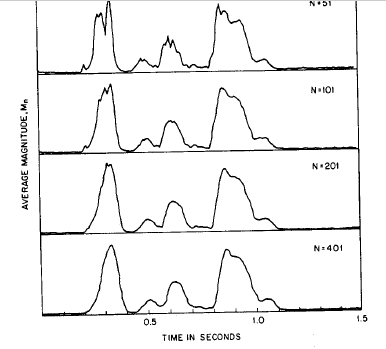
\includegraphics[width=0.5\linewidth]{figures/promedioHamming}
	\caption{Promedio de magnitud con ventana Hamming}
	\label{fig:promedioHamming}
\end{figure}

\subsubsection{Cruces por cero}

En señales discretas en tiempo, un cruce por cero se dice que ocurre si muestras sucesivas tienen diferente signo algebraico. La velocidad a la cual los cruces por cero ocurren es una simple medida del contenido de frecuencia de una señal. Esto es particularmente cierto en señales de banda estrecha. Por ejemplo, una señal sinusoidal de frecuencia $f_0$ muestreada a una tasa $f_s$, tiene $\frac{f_s}{f_0}$  muestras por periodo de la señal sinusoidal. Cada periodo tiene dos cruces por cero así que la tasa promedio de cruces por cero es:

\begin{equation}\label{eq:promedio}
	Z=2\frac{f_0}{f_s}
\end{equation}
Donde:
\\$Z->$ tasa promedio de cruces por cero de una señal sinusoidal.

Así, el promedio de la tasa de cruces por cero da una vía razonable para estimar la frecuencia de la señal sinusoidal.

Señales de voz son señales de banda ancha y la interpretación del promedio de la tasa de cruces es por lo tanto mucho menos precisa. Como sea, estimaciones aproximadas de las propiedades espectrales se pueden obtener usando una representación basada en el promedio de la tasa de cruces por cero en tiempo corto. Una definición apropiada del promedio de cruces por cero está dada por:


\begin{equation}\label{eq:zeroCross}
	Z_n=\sum_{m=-\infty}^{\infty}{|sgn[x(m)]-sgn[x(m-1)]|w(n-m)}
\end{equation}

Donde

\begin{equation}\label{eq:promedio}
	sgn[x(n)]= 
\begin{cases}
    1,	& x(n)\geq0\\
    -1,              & x(n)<0
\end{cases}
\end{equation}

y

\begin{equation}\label{eq:promedio}
	w(n)= 
\begin{cases}
    \frac{1}{2N},	& 0\leq n\leq N-1\\
    -1,              & \text{otro caso}
\end{cases}
\end{equation}

Las operaciones de (\ref{eq:zeroCross}) están representadas en un diagrama de bloques de la Figura \ref{fig:crucesCero}.

\begin{figure}[H]
	\centering
	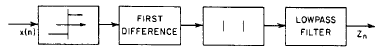
\includegraphics[width=0.6\linewidth]{figures/crucesCero}
	\caption{Diagrama a bloques del cálculo de cruces por cero}
	\label{fig:crucesCero}
\end{figure}

La representación muestra que el promedio de la tasa de cruces por cero en tiempo corto tiene las mismas propiedades generales que el promedio de energía y magnitud en tiempo corto.

El modelo de producción de la voz sugiere que la energía de la señal sonora está concentrada por debajo de los 3kHz, mientras que, para señales no sonoras, la mayor parte de la energía se encuentra en altas frecuencias. Desde altas frecuencias implica altas tasas de cruce por cero, y bajas frecuencias implican bajas tasas de cruce por cero, hay una fuerte correlación entre tasa de cruces por cero y distribución de energía con frecuencia. Una generalización es que, si la tasa de cruces por cero es alta, la señal de voz es no sonora, mientras que, si la tasa de cruces por cero es baja, la señal de voz es sonora. Esto, sin embargo, esta declaración es muy imprecisa porque no se tiene una forma de decir qué es alto y qué es bajo.

En la Figura \ref{fig:gaussianHisto} se muestra un histograma del promedio de la tasa de cruces por cero para señal sonora y no sonora. La media del promedio de la tasa de cruces por cero en tiempo corto es de 49 cada 10 ms para señal no sonora y 14 cada 10 ms para sonora. Claramente las dos distribuciones se traslapan por lo que una decisión inequívoca de sonora y no sonora no es posible basado únicamente en el promedio de cruces por cero en tiempo corto.

\begin{figure}[H]
	\centering
	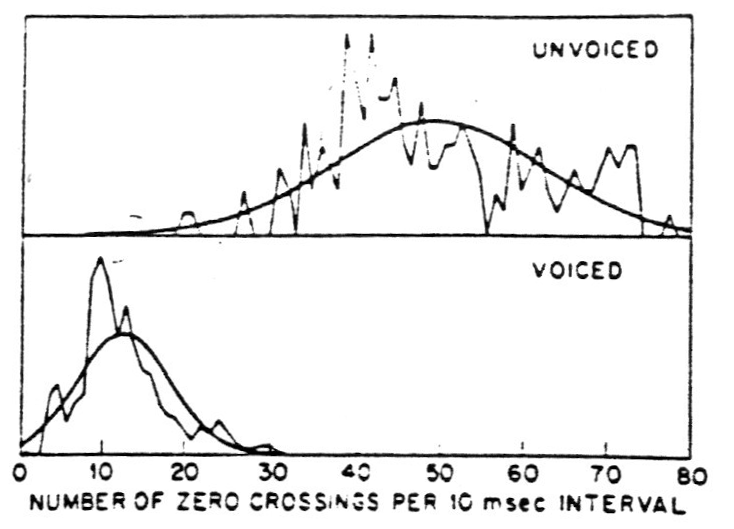
\includegraphics[width=0.6\linewidth]{figures/gaussianHisto}
	\caption{Cruces por cero en un intervalo de 10 ms}
	\label{fig:gaussianHisto}
\end{figure}

La aplicación del procesamiento de voz a cualquier tarea requiere el entendimiento previo de las características de la voz y el tratamiento que se le debe dar de acuerdo al fin que se desee. En particular para el reconocimiento del habla, el esquema de procesamiento que se sigue es similar al presentado en la Figura \ref{fig:esquemaReconocimiento}.

\begin{figure}[H]
	\centering
	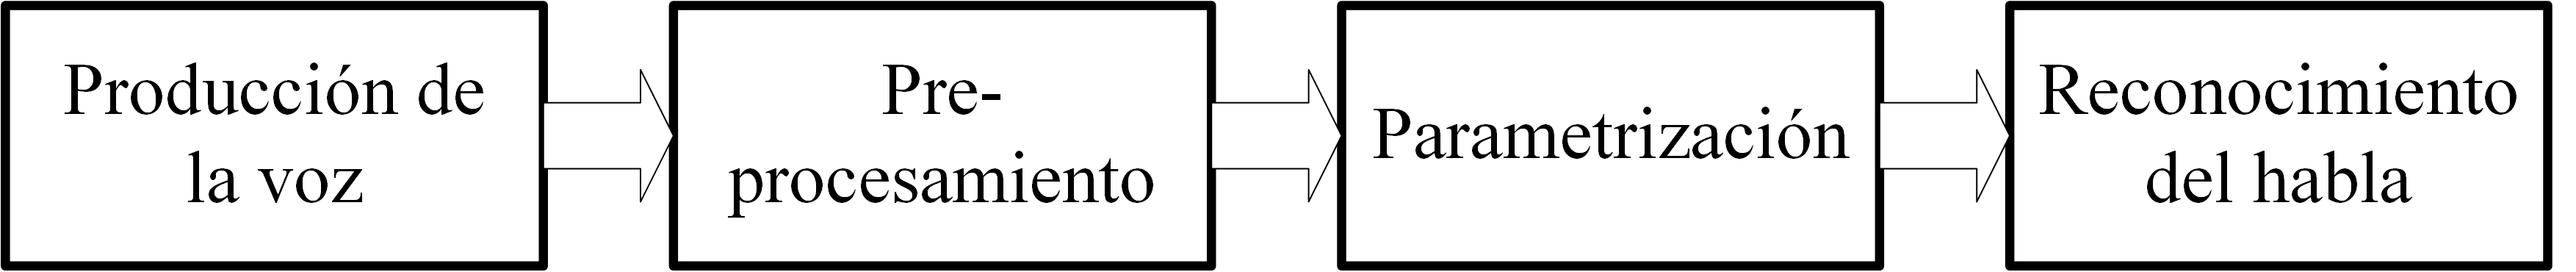
\includegraphics[width=0.8\linewidth]{figures/esquemaReconocimiento}
	\caption{Esquema general del reconocimiento de voz}
	\label{fig:esquemaReconocimiento}
\end{figure}

Es necesario entender las bases para llevar a cabo el reconocimiento de voz, para esto, se describen los bloques presentados en la Figura \ref{fig:esquemaReconocimiento}, lo cual nos llevará a decidir las mejores técnicas a emplear para llevar a cabo este proceso. \cite{SalcedoCherubini2006}

\subsection{Pre-procesamiento}

La etapa de pre-procesamiento corresponde a los pasos previos a la parametrización de la señal de voz, estos pasos son necesarios para resaltar las características más importantes y posteriormente analizarlas con las técnicas de parametrización. La Figura \ref{fig:preProcesamiento} muestra el diagrama a bloques del pre-procesamiento propuesto.

\begin{figure}[H]
	\centering
	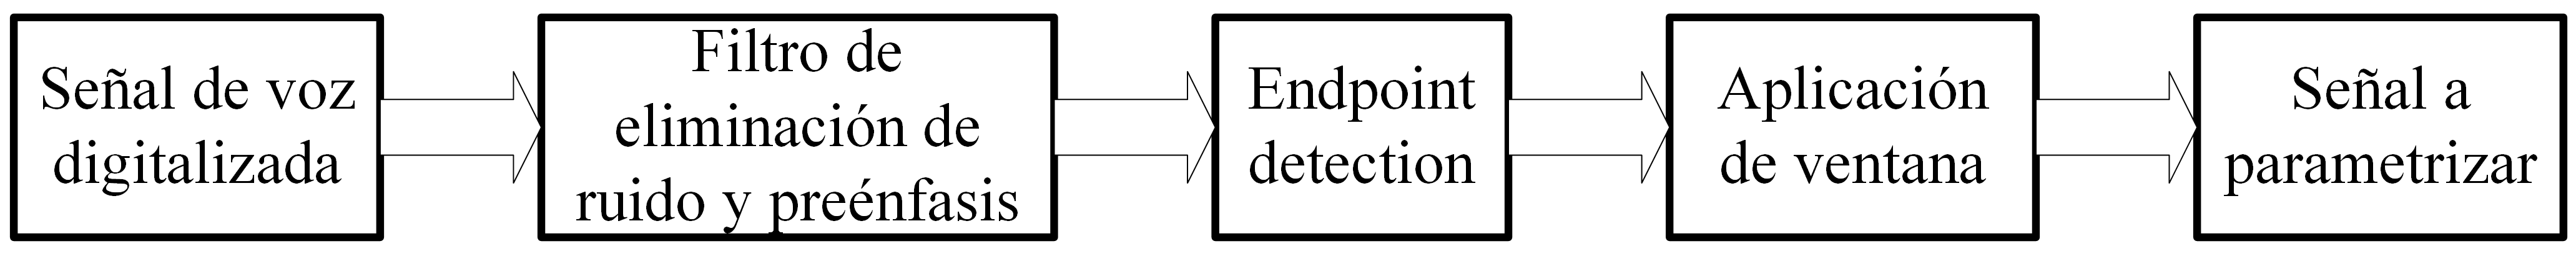
\includegraphics[width=0.9\linewidth]{figures/preProcesamiento}
	\caption{Diagrama a bloques del pre-procesamiento}
	\label{fig:preProcesamiento}
\end{figure}

A continuación, se detalla cada bloque presentado en la Figura \ref{fig:preProcesamiento}. Cabe mencionar que la señal de voz digitalizada, es el resultado de los procesos de adquisición de la voz a través del micrófono y la conversión analógica-digital.

\subsubsection{Filtro preénfasis}

La etapa de preénfasis se realiza para hacer el procesamiento de la señal menos susceptible a truncamientos, aplanarla espectralmente y compensar la caída de 6dB que experimenta la señal al pasar a través del tracto vocal. Generalmente se usa un filtro digital de primer orden cuya función de transferencia es la que se muestra en la ecuación (\ref{eq:preenfasis}). \cite{SalcedoCherubini2006}

\begin{equation}\label{eq:preenfasis}
	H(z)=1-az^{-1}
\end{equation}

Donde a toma valores entre [0.9, 0.95], valor cercano a la unidad a fin de que la estructura de los formantes mayores sea acentuada. La salida de la etapa de preénfasis está dada por la ecuación (\ref{eq:salidaPreenfasis}).

\begin{equation}\label{eq:salidaPreenfasis}
	\tilde{s}(n)=s(n)-a\cdot s(n-1)
\end{equation}

Donde:
\\$\tilde{s}->$ señal filtrada.
\\$s->$ señal de voz.

\subsubsection{Endpoint detection}

Un problema importante en el procesamiento del habla es el detectar la presencia del habla en un ambiente ruidoso. Este problema es comúnmente conocido como \textit{endpoint location problem}. La detección precisa del inicio y fin de una palabra significa que el procesamiento posterior se puede mantener a un mínimo logrando optimizar recursos.

Una de las principales causas de los errores en sistemas de reconocimiento del habla en palabras aisladas es la detección inexacta de los límites inicial y final en los patrones de prueba y de referencia. Es esencial en los sistemas de reconocimiento automático del habla que los segmentos de habla puedan separarse de forma fiable de los segmentos de no habla.

Requerimientos del algoritmo:

\begin{itemize}
\item	Fiabilidad y robustez: el endpointer sin supervisión automática debe ser fiable, es decir, lo suficientemente robusta como para evitar errores de clasificación en las condiciones de trabajo difíciles, tales como la variación de la relación señal a ruido, intensidad variable, etc.
\item	Precisión: Mínima pérdida de segmentos como los siguientes no es admisible
\begin{itemize}
\item	Inicio o término de palabras con fonemas de baja energía.
\item	Oclusiva sorda.
\item	Una nasal.
\item	Una respiración corta, golpe, o ligero ruido.
\end{itemize}
\item	Adaptabilidad: el algoritmo debe ser adaptivo para ser capaz de hacer frente a los cambios del entorno, especialmente el ruido de fondo variable.
\item	Simplicidad: la simplicidad es otra característica deseada de especial importancia cuando el algoritmo está pensado como parte del reconocedor. Por ejemplo, los algoritmos que manejan condiciones difíciles tales como el habla de telefonía suelen ser muy compleja.
\item	Procesamiento en tiempo real: también se desea el procesamiento en tiempo real y sólo es posible si el algoritmo no es complejo.
\item	No conocimiento a priori de ruido: se requiere en un algoritmo ideal que debe ser capaz de hacer frente a la variación de la relación señal a ruido.
\end{itemize}

El algoritmo propuesto en \cite{Rabiner1975} usa dos medidas de la señal, la energía y la tasa de cruces por cero.

Tres umbrales se calculan:

\begin{itemize}
\item	ITU – Upper energy threshold
\item	ITL – Lower energy threshold
\item	IZCT – Zero crossings rate threshold
\end{itemize}

\subsubsection{Aplicación de ventana}

En la etapa siguiente, la señal filtrada y sin silencios, obteniendo así la información útil de la voz, se hace necesario dividir la señal en tramas de N muestras, donde N es un valor que se escoge tomando en cuenta que la señal de voz es estacionaria a segmentos; condición necesaria para realizar el análisis de Fourier en tiempo corto. El intervalo de tiempo en el que la señal de voz se considera estacionaria depende de la velocidad de cambios del tracto vocal y las cuerdas vocales, comúnmente se establece un valor entre 20 y 40 ms. \cite{SalcedoCherubini2006}

En la Figura \ref{fig:segmentacion} se muestra un ejemplo de segmentación utilizado comúnmente en las aplicaciones de procesamiento de voz. Por lo general se utilizan tramas de 256 muestras por ser un valor que establece un equilibrio entre la resolución en tiempo y frecuencia para una señal de voz.

\begin{figure}[H]
	\centering
	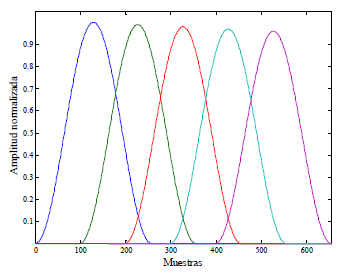
\includegraphics[width=0.6\linewidth]{figures/segmentacion}
	\caption{Segmentación de la señal de voz en tramas solapadas entre ellas.}
	\label{fig:segmentacion}
\end{figure}

Para esta fase del pre-procesamiento es importante escoger la ventana más adecuada que vamos a aplicar a nuestras tramas, para esta decisión es importante tener en cuenta el efecto de ésta sobre la resolución espectral de la señal, la cual depende del lóbulo central y la atenuación de los lóbulos laterales. Lo ideal es que el lóbulo central sea muy estrecho y los lóbulos laterales sean lo más pequeño posible.

En la Figura \ref{fig:windows} se muestran cuatro ventanas con su respectivo espectro, en la cual es fácil observar cómo es la relación del lóbulo central con sus lóbulos laterales, así como también la etnuación que tienen éstos últimos, podemos observar que la ventana de Blackman es la que presenta mayor atenuación en los lóbulos laterales con el precio de que el lóbulo central  es más ancho que las demás ventanas.

\begin{figure}[H]
	\centering
	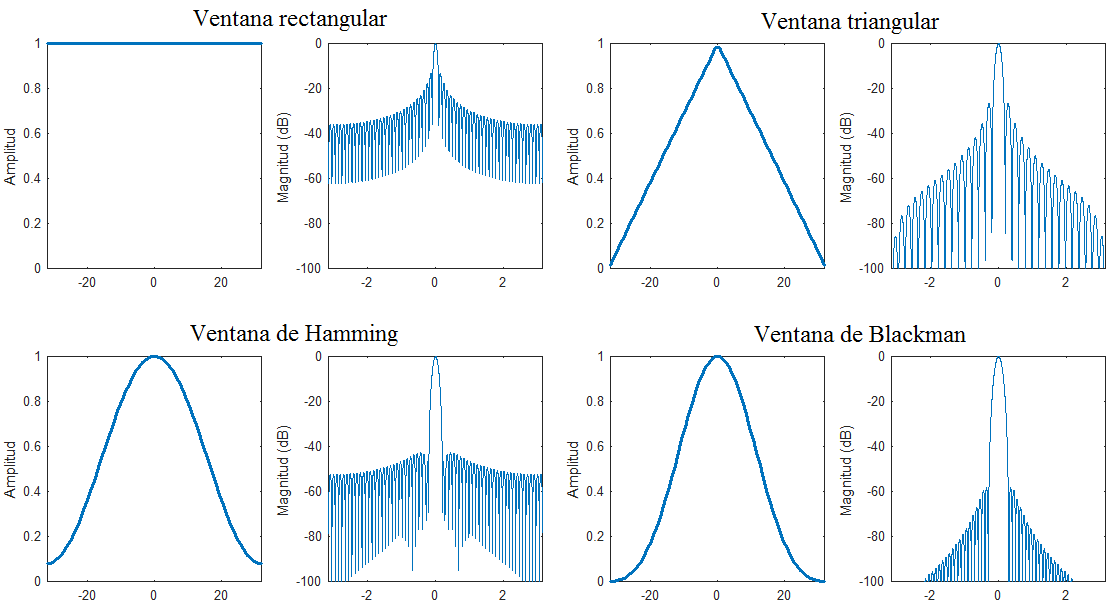
\includegraphics[width=1\linewidth]{figures/windows}
	\caption{Ventanas en el dominio del tiempo y la frecuencia.}
	\label{fig:windows}
\end{figure}

Las ventanas, tanto rectangulares y no rectangulares tienen sus ventajas y desventajas, pero dado los criterios mencionados, en el campo del procesamiento de voz la ventana de Hamming es muy utilizada, pues cumple con el requerimiento de que los lóbulos laterales sean pequeños, a pesar de que su lóbulo central es más ancho que para la ventana rectangular. La ventana de Hamming se define de acuerdo a la ecuación (\ref{eq:hammingWindow})

\begin{equation}\label{eq:hammingWindow}
	W(nT)=0.54-0.46\cdot cos(2\cdot \frac{n}{N})
\end{equation}

Donde $0<n<N$

Un aspecto importante a analizar es el solapamiento de las ventanas entre tramas consecutivas, para la Figura \ref{fig:segmentacion} es de 156 muestras y esto se lleva a cabo por dos propósitos: el primero consiste en que las mismas guarden relación entre sí para que el análisis de cada trama no sea aislado y el segundo consiste en compensar el hecho de que para la ventana de Hamming, la mayor concentración de energía se encuentra en el centro de la trama n y para compensar la caída que tiene la ventana en los bordes de la trama, se utiliza la ventana aplicada en la trama n+1. \cite{SalcedoCherubini2006}

\subsection{Parametrización}

Para cualquier sistema de reconocimiento de voz es importante hacer la selección de la mejor representación paramétrica de la señal de voz, el objetivo principal de esta representación es comprimir los datos correspondientes a la señal eliminando información no pertinente al análisis fonético de la información y extraer las características de la señal que contribuyen a la detección de las diferencias fonéticas que no son apreciables mediante un análisis en tiempo o frecuencia, para esto se hace un análisis más exhaustivo como el Cepstrum. \cite{SalcedoCherubini2006}

\subsubsection{Cepstrum}

El Cepstrum es comúnmente utilizado para la representación paramétrica de señales de voz, desde un punto de vista matemático, se puede decir que se trata de un operador que transforma una convolución en el tiempo en una suma en el dominio espectral. Consiguiendo separar de una forma elegante las dos componentes de información de la señal de voz: la excitación y el tracto vocal. \cite{David2012}

El Cepstrum se define como la transformada inversa de Fourier del logaritmo del espectro de la señal de voz, ecuación (\ref{eq:cepstrum}).

\begin{equation}\label{eq:cepstrum}
	Cepstrum(s[n])=\hat{s}[n]=F^{-1}[log(|F[s[n]]|)]
\end{equation}

En donde s[n] representa la convolución entre la excitación y el tracto vocal:

\begin{equation}\label{eq:conv}
	s[n]=e[n]*h[n]
\end{equation}

Aunque casi todas las técnicas paramétricas de extracción de características de la señal de voz hacen uso de Cepstrum, ésta raramente se utiliza directamente debido a su alta vulnerabilidad con los efectos del canal. Además, para mejorar la eficiencia del sistema, resulta útil intentar emular el comportamiento frecuencial del oído humano, para esto se hace uso de una nueva escala de frecuencia no lineal denominada MEL para imitar el comportamiento psicoacústico a tonos puros de distinta frecuencia dentro del oído humano. \cite{David2012}

\subsubsection{LPCC (Linear-Prediction Cepstral Coefficients)}

La técnica LPCC permite estimar los coeficientes cepstrales mediante el uso del algoritmo LPC, que establece un modelo que permite calcular la próxima muestra de la señal mediante la función de transferencia que se muestra en la ecuación (\ref{eq:transfLPC})

\begin{equation}\label{eq:transfLPC}
	H(z)=\frac{G}{1-\sum_{k=1}^{p}{a_k\cdot z^{-k}}}
\end{equation}

Donde G es la ganancia del filtro, que depende de la señal y $a_k$ son los coeficientes del filtro que modela el tracto vocal.

Este análisis se basa en la Figura \ref{fig:modeloSimplificado} y la idea fundamental es que la voz puede modelarse a través de una combinación lineal de p muestras anteriores más una señal de excitación (periódica o ruido blanco dependiendo de la naturaleza de la señal, como se muestra en la ecuación (\ref{eq:comLin}).

\begin{equation}\label{eq:comLin}
	s[n]=\sum_{k=1}^{p}{a_k\cdot s[n-k]+G\cdot u[n]}
\end{equation}

Donde u[n] es la entrada del filtro que modela el tracto vocal, por lo que, dada la señal s[n], el problema consiste en determinar los coeficientes de predicción $a_k$ y la ganancia G del filtro.

Los coeficientes de predicción se usan en el proceso de parametrización para calcular los coeficientes cepstrales, por lo tanto, dada una señal s[n] un predictor de orden p se puede definir como lo muestra la ecuación (\ref{eq:predictor}).

\begin{equation}\label{eq:predictor}
	\tilde{s}[n]=-\sum_{k=1}^{p}{a_k\cdot s[n-k]}
\end{equation}

Para determinar los coeficientes de predicción $a_k$ se minimiza el error de predicción de orden p representado por la ecuación (\ref{eq:minError}).

\begin{equation}\label{eq:minError}
	e[n]=s[n]-\tilde{s}[n]
\end{equation}

Donde e[n] es la señal de error, los coeficientes de predicción se calculan minimizando la media del error cuadrático medio con respecto a cada uno de los coeficientes, ecuación (\ref{eq:cuaMedio})

\begin{equation}\label{eq:cuaMedio}
	\tilde{e}=E\left \{e^2[n]\right \}
\end{equation}

Para obtener el mínimo de error de predicción se calcula la derivada de e[n] con respecto a los coeficientes $a_k$, obteniendo la ecuación (\ref{eq:derivada})

\begin{equation}\label{eq:derivada}
	\sum_{k=1}^{p} {a_k\cdot E\left \{  s[n-k]\cdot s[n-i] \right \}} = -E\left \{ s[n]\cdot s[n-i]\right \}, 1<i<p
\end{equation}

El error de predicción mínimo viene definido por (\ref{eq:eCuaMedio})

\begin{equation}\label{eq:eCuaMedio}
	\tilde{e}_{min}=E\left \{ y^2[n]\right \} +\sum_{k=1}^{p}{a_k\cdot E\left \{ y[n]\cdot y[n-k]\right \}}
\end{equation}

Por (\ref{eq:eCuaMedio}) podemos escribir el error cuadrático medio mínimo en función de la autocorrelación (\ref{eq:corr}).

\begin{equation}\label{eq:corr}
	\tilde{e}_{min}=R(0)+\sum_{k=1}^{p}{a_k\cdot R(k)}
\end{equation}

Estas ecuaciones son llamadas ecuaciones normales o de Yule-Walker y los coeficientes $a_k$ del predictor óptimo se obtienen resolviendo las \textit{p} ecuaciones con \textit{p} incógnitas. \cite{SalcedoCherubini2006}

En \cite{SalcedoCherubini2006} se muestra como resultado del análisis que mediante el uso de LPC como técnica de predicción lineal, de todos los posibles parámetros que se pueden obtener a partir del modelado de la voz como un proceso autorregresivo, los coeficientes $a_k$ que modelan el tracto vocal, pueden ser utilizados para el cálculo de los coeficientes cepstrales o LPCC’s mediante (\ref{eq:coefTracto})

\begin{equation}\label{eq:coefTracto}
	c_i=a_i+\sum_{K=1}^{i-1}(\frac{k-i}{i})\cdot c_{i-k}\cdot a_k
\end{equation}

Se puede observar cómo la predicción de los coeficientes del filtro que modelan el tracto vocal puede ser utilizada para estimar por ejemplo la densidad espectral de potencia de la señal de voz o como en el presente caso, estimar los coeficientes cepstrales utilizados en el reconocimiento del habla.

\subsubsection{MFCC (Mel-Frequency Cepstral Coefficients)}

El objetivo de los MFCC es obtener una representación compacta, robusta y apropiada para posteriormente poder obtener un modelo estadístico con un alto grado de precisión, en la Figura \ref{fig:mfccB} se muestra el esquema básico para la obtención de los MFCC.

\begin{figure}[H]
	\centering
	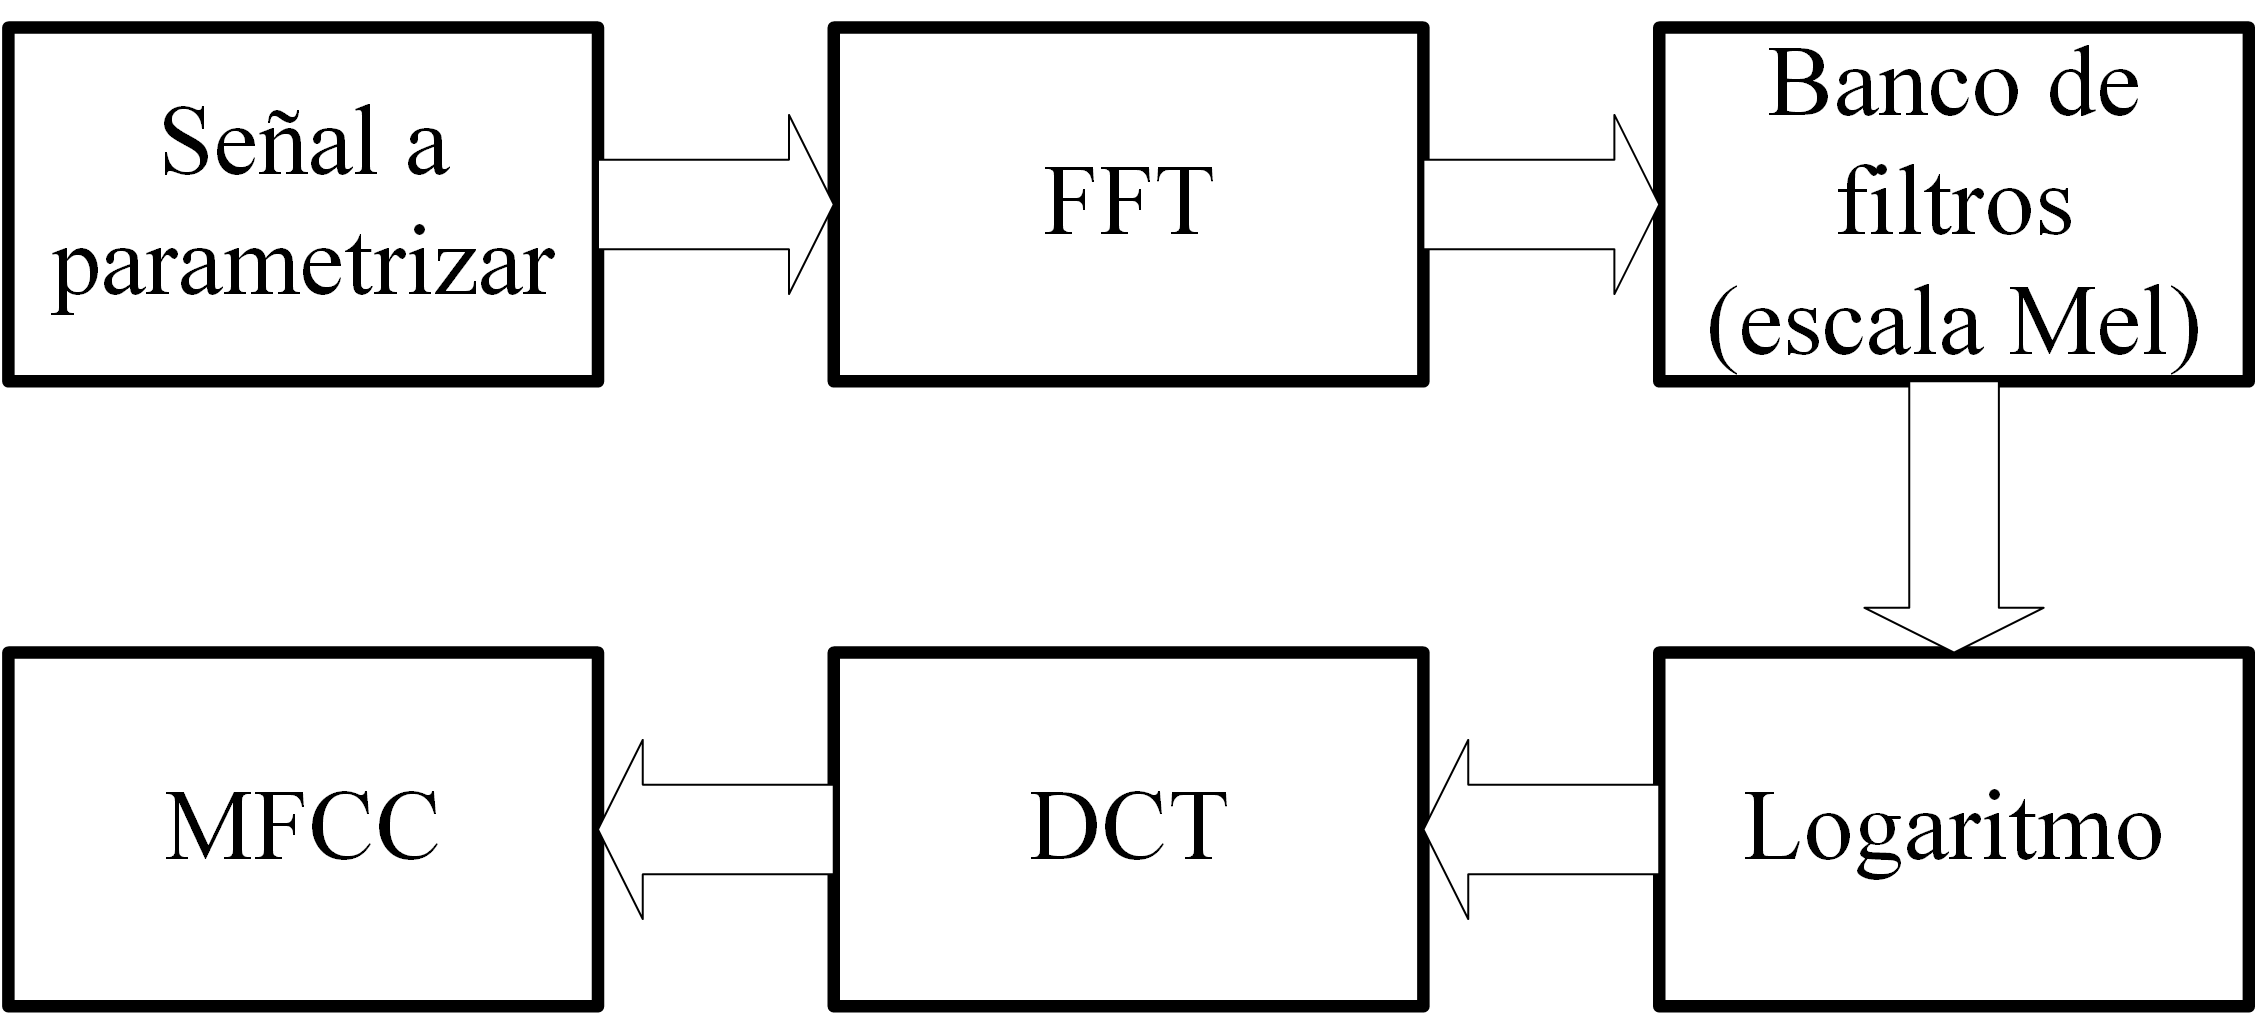
\includegraphics[width=0.6\linewidth]{figures/mfcc}
	\caption{Diagrama a bloques para el cálculo de MFCC}
	\label{fig:mfccB}
\end{figure}

\subsubsection*{FFT}

Se calcula la transformad de Fourier de Tiempo Corto a cada una de las tramas obtenidas de la etapa de pre-procesamiento mediante:

\begin{equation}\label{eq:fftCorto}
	x(n,\omega_k)=\sum_{m=-\infty}^{\infty}{x(m)\cdot w(n-m)\cdot e^{-j\omega_km}}
\end{equation}

Donde: $\omega_k=\frac{2\pi}{N}k$ 

\subsubsection*{Banco de filtros (escala Mel)}

Los filtros que se le aplican a la señal en la técnica MFCC están espaciados linealmente para frecuencias menores a 1000 Hz y logarítmicamente para frecuencias mayores de 1000 Hz. A esta escala se le denomina “Escala Mel” y su fórmula matemática está dada por la ecuación (\ref{eq:filtMEL}).

\begin{equation}\label{eq:filtMEL}
	Mel(f)=2595\cdot log(1+\frac{f}{700})
\end{equation}

El cuadrado de la magnitud de $x(n,\omega_k )$ es ponderado por una serie de filtros distribuidos sobre la escala de Mel para luego calcular la llamada energía del filtro l-ésimo mediante la ecuación (\ref{eq:logEnergia})

\begin{equation}\label{eq:logEnergia}
	E_{Mel}(n,l)=\frac{1}{A_l}\cdot \sum_{k=L_l}^{U_l}{|V_L(\omega_k)\cdot X(n,\omega_k)|^2}
\end{equation}

Donde $L_l$  y $U_l$ son las frecuencias de corte inferior y superior del filtro l-ésimo.

El banco de filtros linealmente espaciado en la escala de Mel tiene la forma que se muestra en la Figura 18 y los filtros que lo conforman pueden ser triangulares o tener otras formas, tales como Hamming, Hanning o kaizer, pero el triangular es el más utilizado.

\begin{figure}[H]
	\centering
	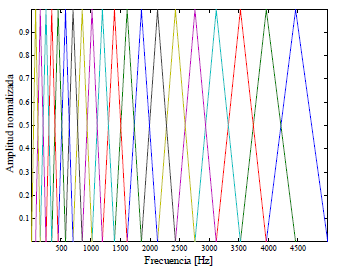
\includegraphics[width=0.6\linewidth]{figures/bancoFiltros}
	\caption{Banco de filtros en la escala de Mel}
	\label{fig:bancoFiltros}
\end{figure}

\subsubsection*{DCT}

Se convierte el espectro logarítmico Mel nuevamente al dominio del tiempo usando la Transformada Discreta del Coseno, dado que los coeficientes cepstrales son reales. El cálculo se realiza con la ecuación (\ref{eq:dct}).

\begin{equation}\label{eq:dct}
	C_{Mel}[n,m]=\frac{1}{R}\cdot \sum_{l=1}^{R}{log\left \{ E_{Mel}(n,l)\right \}\cdot cos[n(l-\frac{1}{2})\cdot \frac{\pi}{l}]}, n=1,2,3,...,K
\end{equation}

Donde K es el número de coeficientes cepstrales, que por lo general se escoge entre 10 y 20.

Mediante el proceso descrito, para cada trama de voz de duración aproximada igual a 30 ms con solapamiento, se calcula un conjunto de coeficientes cepstrales. Este es el resultado de la transformada Discreta de Coseno de la Densidad Espectral de Potencia expresada en la escala de Mel. A este conjunto de coeficientes se denomina Vector Acústico, por lo que cada entrada es transformada mediante este proceso en una secuencia de Vectores acústicos que representan las características más importantes de la voz, necesarias para el reconocimiento del habla. \cite{SalcedoCherubini2006}

\subsubsection{LFCC (Linear-Frequency Cepstral Coefficients)}

El funcionamiento de la obtención de los LFCC’s es similar al proceso de obtención de los MFCC’s, con la única diferencia de que los bancos de filtros utilizados que se le aplican a la señal se encuentran sobre una escala lineal. El banco de filtros que se generan con esta técnica se observa en la Figura \ref{fig:lfcc}.

\begin{figure}[H]
	\centering
	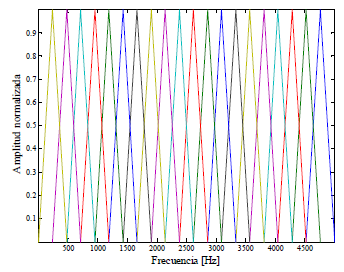
\includegraphics[width=0.6\linewidth]{figures/lfcc}
	\caption{Banco de filtros para el cálculo de LFCC's}
	\label{fig:lfcc}
\end{figure}

Cabe mencionar que la diferencia entre los tres métodos de extracción de características es principalmente que cada uno se utiliza para la extracción de distintas características de la voz.

\subsection{Cuantización vectorial}

El resultado de un análisis por banco de filtros o análisis LPC son una serie de vectores de las características espectrales variables en el tiempo de la señal de voz, donde típicamente cada vector es un vector p-dimensional. \cite{Rabiner1993}

Por esto, en particular para el reconocimiento del habla, la esencia de la cuantización vectorial es la de obtener a partir de un vector cualquiera de coeficientes cepstrales, un vector de tamaño fijo que se parezca lo más posible al original. Para ello, el espacio generado por los coeficientes cepstrales es dividido en un conjunto de regiones convexas mutuamente excluyentes y para cada una se calcula el centroide. El conjunto de centroide obtenidos de la partición del espacio generado por los coeficientes cepstrales se le denomina codebook. Por lo tanto, a cada palabra se la asocia su propio codebook.

La cuantización vectorial presenta ventajas y desventajas mencionadas en \cite{Rabiner1993}:

\begin{itemize}
\item	Ventajas
\begin{itemize}
\item	Reduce el almacenamiento de información de análisis espectral: La eficiencia de la representación de la cuantización vectorial puede ser explotada en sistemas de reconocimiento del habla.
\item	Reducción de cálculo para determinar la similitud de vectores de análisis espectral. En reconocimiento del habla un componente importante de la computación es la determinación de similitud espectral entre un par de vectores.  Basado en la representación de cuantización vectorial, este cálculo de similitud espectral es con frecuencia reducido a una búsqueda en la tabla de similitudes entre pares de vectores codebooks.
\item	Representación discreta de los sonidos del habla. Asociando una etiqueta fonética con cada vector codebook, el proceso de elegir el mejor vector codebook para representar un vector espectral dado llega a ser equivalente a asignar una etiqueta fonética a cada segmento espectral de voz. Existe una gama de sistemas de reconocimiento que explotan estas etiquetas con el fin de reconocer el habla de manera eficiente.
\end{itemize}
\item	Las desventajas de usar la cuantización vectorial para representar un vector espectral de voz son:
\begin{itemize}
\item	Una distorsión espectral inherente en la representación del vector de análisis actual. Ya que sólo hay un número finitos de vectores codebooks, el proceso de elegir la “mejor” representación de un vector espectral dado es equivalente a cuantizar el vector y conduce, por definición, a un cierto nivel de error de cuantización.
\item	El almacenamiento requerido por los vectores codebooks es con frecuencia no trivial. Cuanto más grande hacemos el codebook (con el fin de reducir el error de cuantización), más es el almacenamiento requerido para las entradas codebook.
\end{itemize}
\end{itemize}

\subsubsection{Elementos de la implementación de un cuantizador vectorial}

Para crear un cuantizador vectorial e implementar un procedimiento de análisis, necesitamos lo siguiente:

\begin{enumerate}
\item	Un gran conjunto de vectores de análisis espectral, que conforman el conjunto de entrenamiento. El conjunto de entrenamiento es usado para crear el “óptimo” conjunto de vectores codebook para representar la variabilidad espectral observada en el conjunto de entrenamiento. Si indicamos el tamaño de cuantizador vectorial como $M=2^B$ vectores (a esto se le llama un codebook de B bits), entonces requerimos $L>>M$ de manera que sea capaz de encontrar el mejor conjunto de M vectores codebook de manera robusta. En la práctica, se ha encontrado que L puede ser al menos 10M para que el entrenamiento del cuantizador vectorial trabaje razonablemente bien.
\item	Una mediad de similitud, o distancia, entre un par de vectores de análisis espectral de manera que sea capaz de agrupar el conjunto de vectores de entrenamiento, así como también asociar o clasificar arbitrariamente vectores espectrales en entradas únicas del codebook.
\item	Un procedimiento de cálculo de centroide. Sobre la base de la partición que clasifica los L conjuntos de vectores de entrenamiento en M grupos que, elegimos los M vectores codebook como el centroide de cada uno de los M grupos.
\item	Un procedimiento de clasificación de vectores de análisis de voz espectral arbitrarios que selecciona el vector codebook cercano al vector de entrada y usa el índice del codebook como resultado de representación espectral.
\end{enumerate}

La Figura \ref{fig:vectorQTS} muestra un diagrama de bloques del entrenamiento básico de un cuantificador vectorial y estructura de clasificación.

\begin{figure}[H]
	\centering
	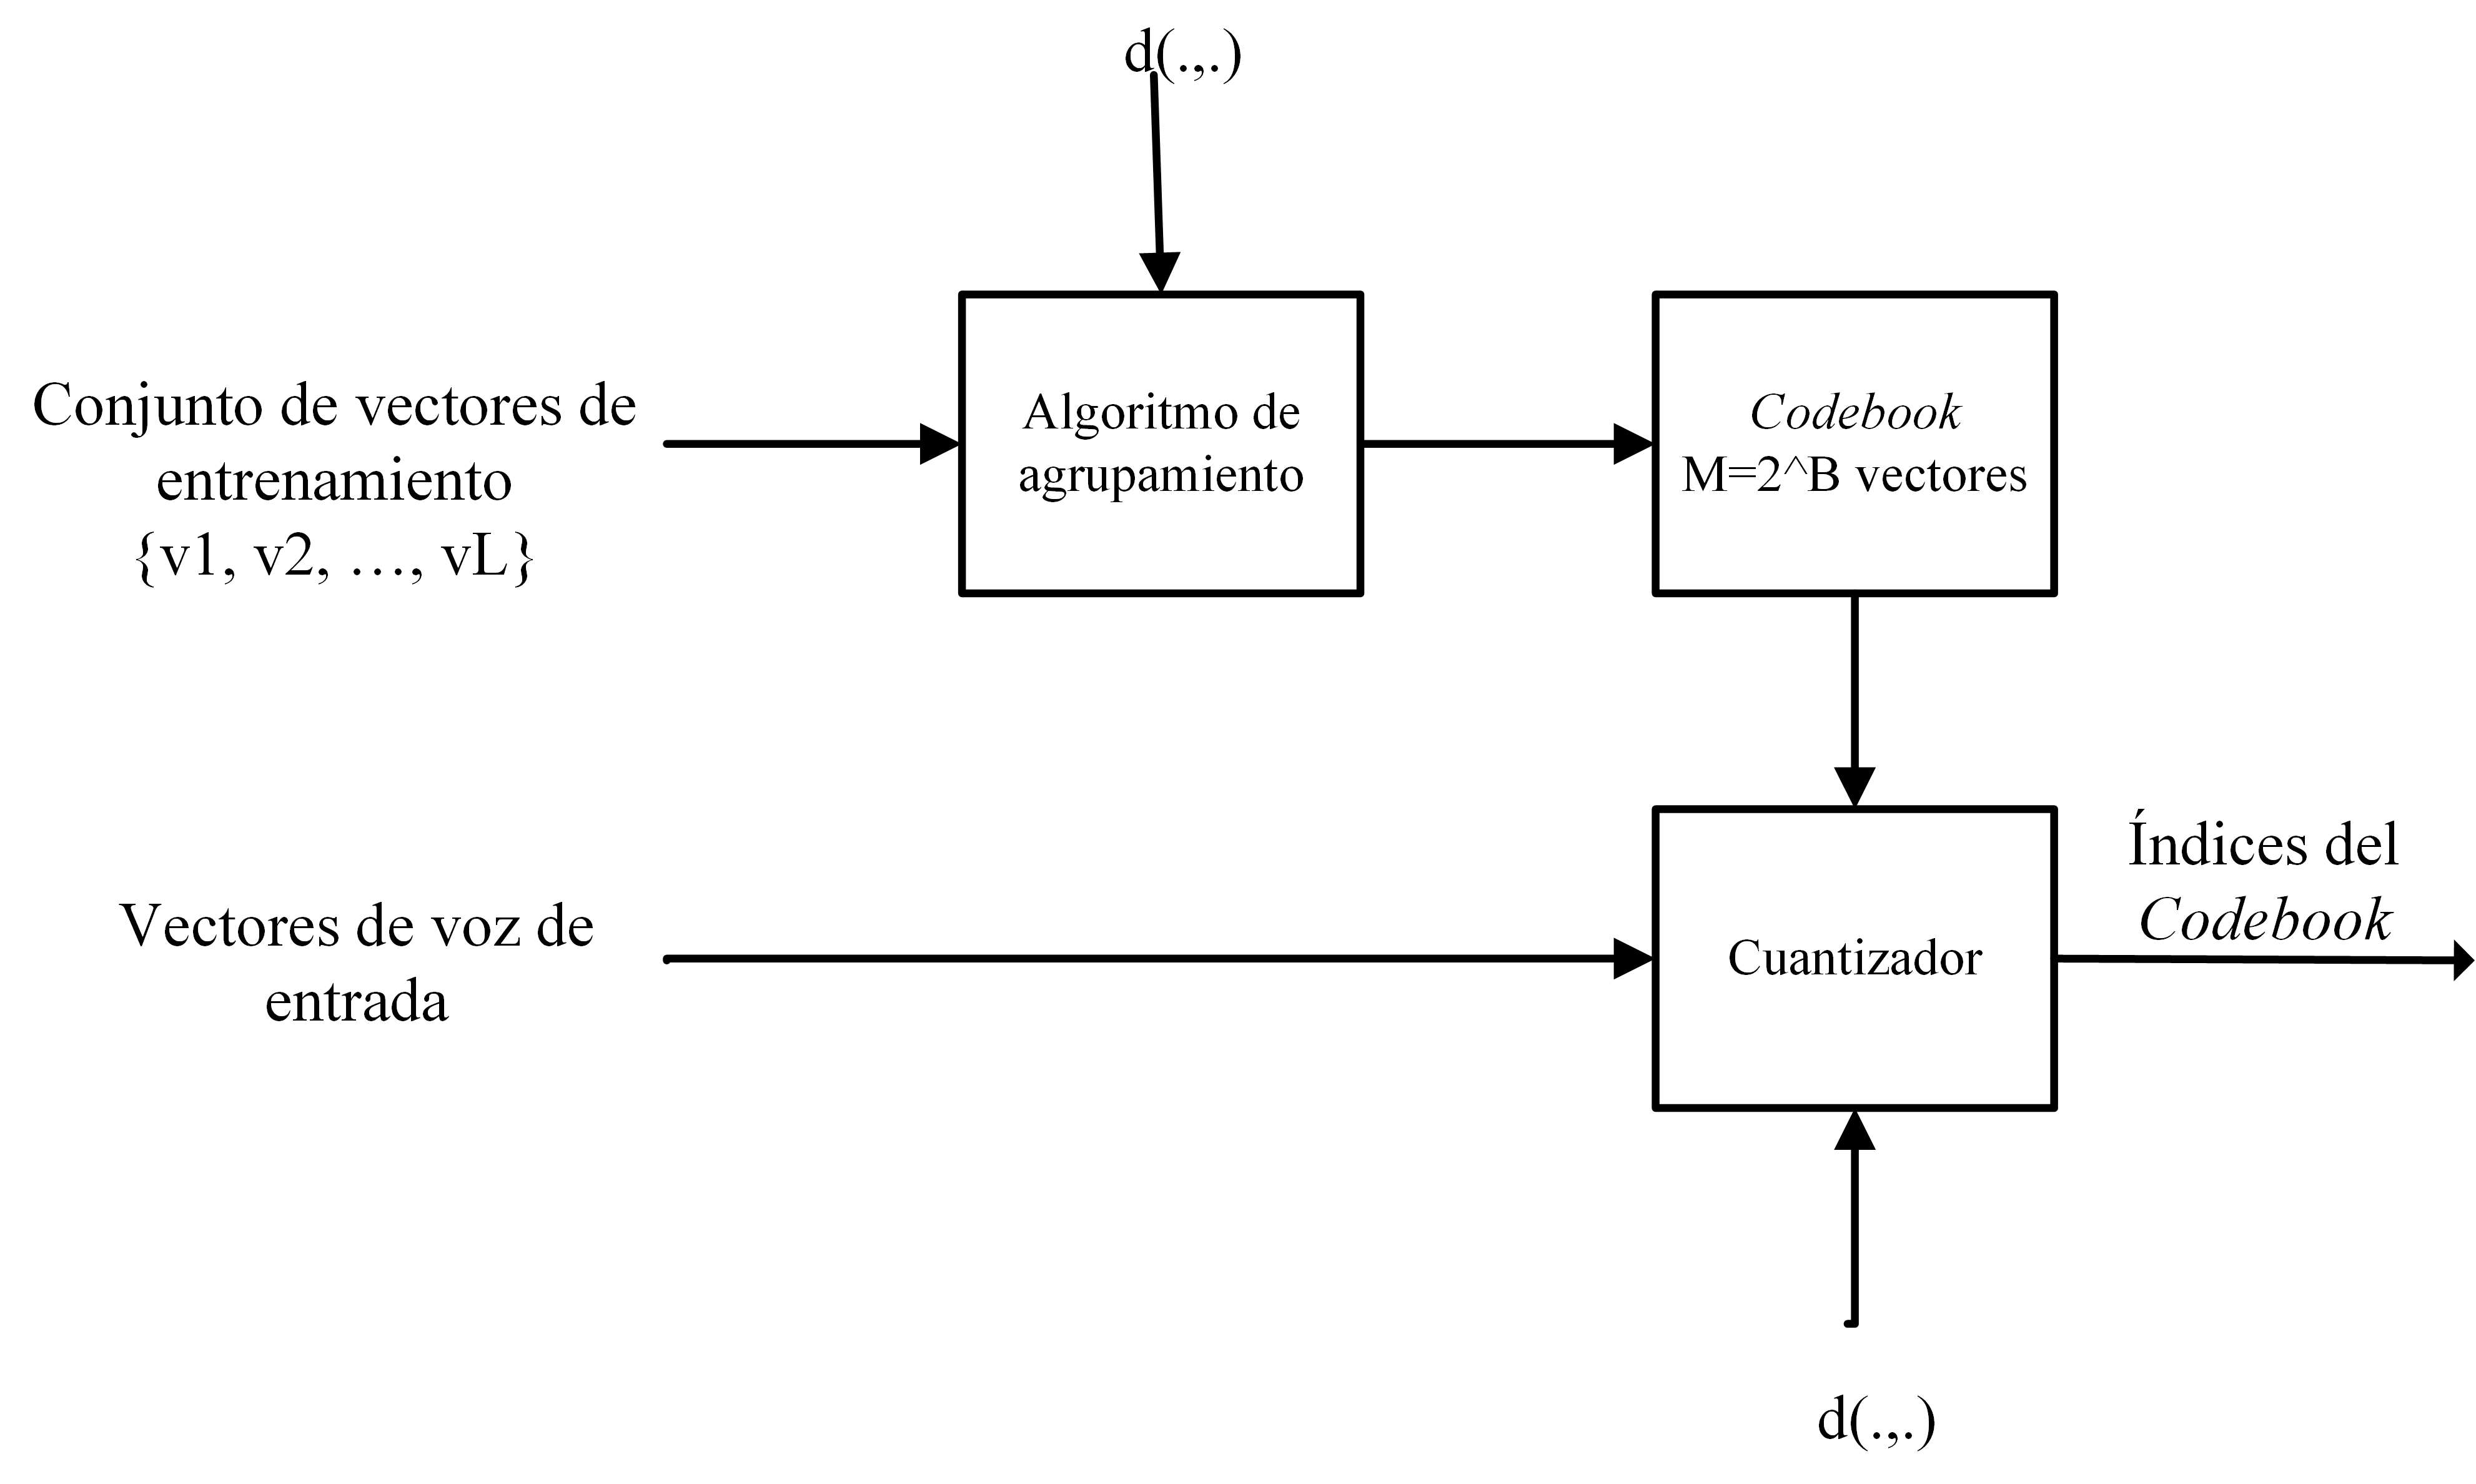
\includegraphics[width=0.6\linewidth]{figures/vectorQTS}
	\caption{Diagrama a bloques del entrenamiento básico de un cuantificador vectorial y estructura de clasificación}
	\label{fig:vectorQTS}
\end{figure}

\subsubsection{El conjunto de entrenamiento del cuantizador vectorial}

Para entrenar apropiadamente el \textit{codebook}, el conjunto de vectores de entrenamiento debe abarcar anticipadamente los siguientes puntos:

\begin{itemize}
\item	Interlocutores, incluyendo rangos de edad, acento, genero, velocidad de habla, nivel y otras variables.
\item	Condiciones de habla, tales como una habitación silenciosa, automovil, área de trabajo ruidosa.
\item	Transductores y sistemas de transmisión, incluyendo micrófonos de banda ancha, transmisión directa, canal telefónico, ancho de banda del canal y otros dispositivos.
\item	Fonemas, vocabulario de reconocimiento.
\end{itemize}

\subsubsection{Agrupación de los vectores de entrenamiento.}

La manera en que el conjunto de L vectores de entrenamiento puede ser agrupados en un conjunto de M vectores codebook es el siguiente (este procedimiento es conocido como el algoritmo generalizado de Lloyd o el algoritmo de agrupación K-means):

\begin{enumerate}
\item	Inicialización: Arbitrariamente elige M vectores (inicialmente fuera del conjunto de entrenamiento de L vectores) como el conjunto inicial de codewords en el codebook.
\item	Buscar el vecino más cercano: Para cada vector de entrenamiento encontrar el codeword en el actual codebook más cercano (en términos de distancia espectral), y asigna ese vector a la celda correspondiente (asociada con el codeword más cercano).
\item	Actualiza el centroide: Actualiza el codeword en cada celda usando el centroide del vector de entrenamiento asignado a esa celda.
\item	Iteración: Repetir paso 2 y 3 hasta que la distancia media cae por debajo del presente umbral.
\end{enumerate}

La Figura \ref{fig:partitioningVectorSpace} ilustra el resultado del diseño de el \textit{codebook} mostrando la partición del espacio vectorial espectral en distintas regiones, cada uno representado por el centroide del vector

\begin{figure}[H]
	\centering
	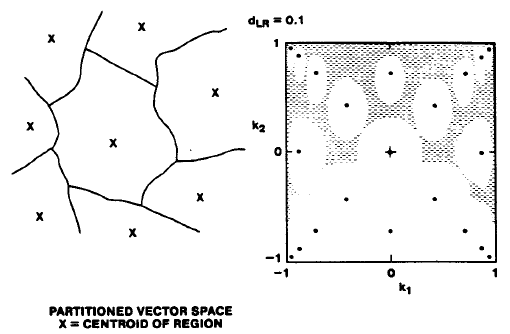
\includegraphics[width=0.6\linewidth]{figures/partitioningVectorSpace}
	\caption{Partición de un espacio vectorial en celdas de cuantización vectorial con cada celda representada por el centroide del vector}
	\label{fig:partitioningVectorSpace}
\end{figure}
	
Aunque el procedimiento iterativo mostrado funciona correctamente, ha sido demostrado que es ventajoso diseñar un codebook de M vectores en etapas, por ejemplo, primero diseñando un codebook de 1 vector, entonces usar la técnica de división en el codeword para inicializar la búsqueda de un codebook de 2 vectores, y continuar con el proceso de división hasta el deseado codebook de M vectores. Este procedimiento es llamado el algoritmo de división binaria y es formalmente implementado mediante el siguiente procedimiento.
	
\begin{enumerate}
\item	Diseñar un vector genérico del codebook; éste será el centroide del conjunto entero de vectores de entrenamiento.
\item	Duplicar el tamaño del codebook dividiendo cada codebook existente $y_n$ de acuerdo a la regla

\begin{equation}\label{eq:codebook}
	\begin{cases}
	    y_n^+=y_n(1+\epsilon)\\
			    y_n^-=y_n(1-\epsilon)
\end{cases}
\end{equation}

Donde n varía de 1 al tamaño actual del codebook, y $\epsilon$ es un parámetro de separación (típicamente $\epsilon$ es elegido en el rango $0.01\leq \epsilon \leq 0.05$).
\item	Usar el algoritmo de iteración K-means para conseguir el mejor conjunto de centroides para la división del codebook.
\item	Iterar los pasos 2 y 3 hasta que el codebook de tamaño M esté diseñado.
\end{enumerate}

\subsection{Redes Neuronales Artificiales}

		\subsubsection{Modelo de neurona artificial}

		Las redes neuronales artificiales pretenden emular la red neuronal biológica y se obtiene interconectando neuronas. Para ello se supone un modelo matemático simplificado de la neurona biológica \cite{Faundez2001}.
		
		Este modelo es una generalización del propuesto por McCulloch y Pitts en 1943:

		\begin{equation}\label{eq:ej}
			y = f \left[ \left( \sum_{i=1}^{N}\omega_i*x\left(n-i\right)\right)-b	\right]
		\end{equation}		

		La Figura \ref{fig:neuronaModel} representa el modelo de neurona artificial.

		\begin{figure}[H]
			\centering
			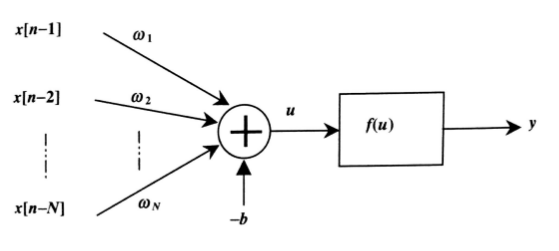
\includegraphics[width=0.6\linewidth]{figures/neuronaA}
			\caption{Modelo de neurona artificial.}
			\label{fig:neuronaModel}
		\end{figure}		

		La neurona recibe del exterior un umbral b y N entradas a las que asocia un conjunto de pesos $\omega_i(i=1,..., N)$. Aplicando el producto de los pesos por las entradas respectivas más el umbral (o desplazamiento) a una función de activación $f(u)$, se obtiene la salida $y$\cite{Faundez2001}.

		$u(\vec{x},\vec{\omega})$ recibe el nombre de función base, donde los vectores $\vec{x}$, $\vec{\omega}$ son:

		\begin{equation}\label{eq:ej}
			\vec{x}=\left\{ x\left[n-1\right],..., \left[n-N\right]	\right\}
		\end{equation}		

		\begin{equation}\label{eq:ej}
			\vec{\omega}=\left\{ \omega_1,..., \omega_N	\right\}
		\end{equation}		

		Cuando la combinación de las entradas es de tipo lineal, $u(\vec{x},\vec{\omega})$ es una función de base lineal, pero son posibles otras combinaciones, entre las que destacan las funciones de base radial, consistentes en realizar una operación no lineal sobre las entradas, con simetría radial. Por ejemplo:

		\begin{equation}\label{eq:ej}
			u\left(\vec{x},\vec{\omega}\right)=\sum_{i=1}^{N}\left[\omega_i-x\left(n-i\right)\right]^2
		\end{equation}		


		La función de activación es la encargada de tomar la decisión de cuándo está activada la neurona y cuándo no, las funciones de activación más comunes se muestran en la Figura \ref{fig:funcionesAct}.

		\begin{figure}[H]
			\centering
			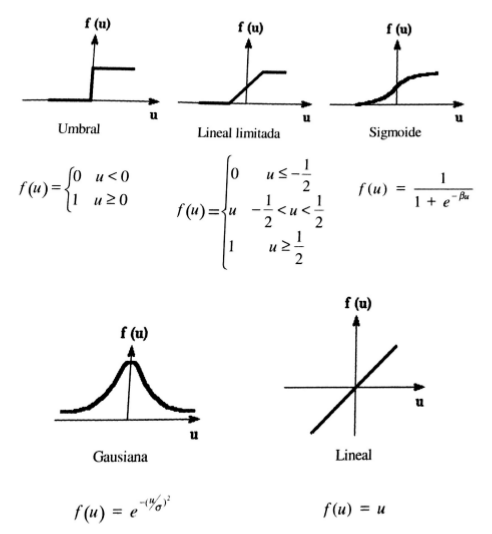
\includegraphics[width=0.6\linewidth]{figures/funcionesAct}
			\caption{Funciones de activación.}
			\label{fig:funcionesAct}
		\end{figure}		

		\subsubsection{Arquitectura de una Red Neuronal Artificial (RNA)}

		Las neuronas de una determinada red pertenecerán a una de las siguientes clases:

		\begin{itemize}
			\item \textbf{Neuronas de entrada:} Reciben las señales exteriores. Integran la primera capa de red.
			\item \textbf{Neuronas ocultas:} Producen resultados intermedios.
			\item \textbf{Neuronas de salida:} Su salida es observable desde el exterior. Constituyen la última capa de la red.
		\end{itemize}

		Por otra parte, dependiendo de la forma en que se encuentren las neuronas y sus conexiones, aparecen dos grandes tipos de redes:
	
		\begin{itemize}
			\item Redes progresivas.
			\item Redes realimentadas.
		\end{itemize}

		En las \textbf{redes progresivas} las conexiones de sus neuronas (y, por lo tanto, el flujo de información) son siempre hacia adelante, de la entrada a la salida. No presentan memoria. Por tanto, son estáticas.

		Las arquitecturas progresivas de mayor importancia son el \textsl{perceptrón} y las redes de función de base radial.

		\begin{figure}[H]
			\centering
			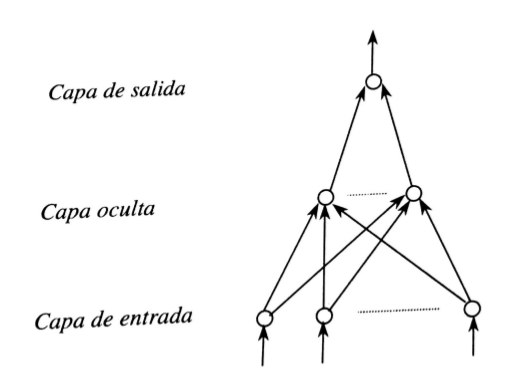
\includegraphics[width=0.8\linewidth]{figures/redProgresiva}
			\caption{Red progresiva.}
			\label{fig:redProgresiva}
		\end{figure}	

		A diferencia de las redes progresivas, las \textbf{redes realimentadas} presentan como mínimo un camino de realimentación, ya sea entre neuronas de una misma capa (conexiones laterales) o como conexión hacia atrás, de una capa exterior a una más interior.

		Son sistemas dinámicos. Cada vez que se presenta una nueva entrada a la red, se calcula la salida de las neuronas. Debido a los lazos de realimentación, las entradas de las neuronas se modifican y la red entra en un nuevo estado \cite{Faundez2001}.

		Las arquitecturas más destacables son:

		\begin{itemize}
			\item Redes competitivas.
			\item Mapas auto organizados de Kohonen.
			\item Red de Hopfield.
			\item Red de Elmann.
			\item Modelos ART.
		\end{itemize}

		\begin{figure}[H]
			\centering
			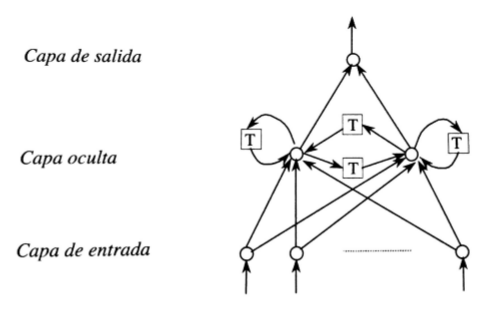
\includegraphics[width=0.8\linewidth]{figures/redRealimentada}
			\caption{Red realimentada.}
			\label{fig:redRealimentada}
		\end{figure}	

		\subsubsection{Aprendizaje}

		Una vez que se establece la arquitectura y el número de neuronas de la red, hay que calcular el valor de los pesos para que realice la función deseada. Usualmente, la red debe aprender el peso de las conexiones a partir de un conjunto de patrones de entrenamiento. Por tanto, no se calculan los pesos de forma analítica, sino que es necesario un proceso de aprendizaje automático  partir de una serie de ejemplos.

		Para diseñar un proceso de aprendizaje será necesario disponer de:

		\begin{itemize}
			\item Un conjunto de información disponible para el aprendizaje.
			\item Un proceso para actualizar los pesos, o algoritmo de aprendizaje.
		\end{itemize}

		\textbf{Aprendizaje supervisado:}
		La red conoce la salida correcta para cada patrón de entrada. Por tanto, se ajustan los pesos de forma que las salidas de la red sean lo más parecidas posibles a la salida correcta.

		\textbf{Aprendizaje por refuerzo:}
		Es una variante del método anterior, en el cual la red únicamente conoce una crítica sobre la exactitud de las salidas, pero no la respuesta correcta.

		Utiliza un mecanismo de penalización y recompensa, mediante el cual la red resulta recompensada por una decisión correcta y castigada por una equivocada. De esta forma, el sistema tiende a actuar de la forma favorecida y debilita la tendencia a proporcionar la respuesta penalizada.

		\textbf{Aprendizaje auto organizado:}
		No requiere el conocimiento de la salida correcta, y debe aprender la estructura implícita en los datos. Generalmente requiere un número mayor de datos de entrenamiento.

		\paragraph{}
		En el aprendizaje, existen tres cuestiones importantes:
		
		\textbf{Capacidad de la red para implementar funciones y aprender patrones.}
		Dependerá de su estructura, tamaño, etc.

		\textbf{Complejidad de los datos.}
		Determina el número de patrones de entrenamiento necesarios para entrenar la red de forma que se garantice una buena capacidad de generalización (capacidad de procesar correctamente datos no utilizados en el aprendizaje). Si el número de patrones es pequeño, la red se comportará bien con aquellos patrones utilizados en el entrenamiento, pero presentará un comportamiento pobre con aquellos datos no utilizados.

		\textbf{Complejidad computacional.}
		Condiciona el tiempo necesario para que el algoritmo de aprendizaje proporcione una solución ajustada.

		El conjunto de patrones utilizados en el proceso de aprendizaje recibe el nombre de secuencia de entrenamiento. Cada vez que se ha presentado la totalidad de la secuencia de entrenamiento a la red, se dice que se ha realizado un ``epoch". Normalmente los algoritmos que consumen poco tiempo en cada epoch requieren muchas epochs y viceversa, con lo cual la evaluación de la complejidad computacional debe considerar el número de epochs necesarios y el tiempo transcurrido en cada epoch \cite{Faundez2001}.

		En la tabla \ref{tabla:aprendizaje} se observan los 3 paradigmas de aprendizaje con sus reglas, arquitectura, algoritmo y tareas correspondientes.

		\begin{table}[H]
			\centering
			\begin{tabular}{| c | p{3cm} | p{3cm} | p{3cm} | p{3cm} |}
				\hline
				\multicolumn{5}{|c|}{Algoritmos de aprendizaje más conocidos} \\
				\hline
				Paradigma	&	Regla de aprendizaje	&	Arquitectura	&	Algortimo de aprendizaje	&	Tareas \\
				\hline \hline
				Supervisado	&	Corrección del error	&	Perceptrón o perceptrón multicapa	&	Algoritmos de aprendizaje perceptrón, retropropagación del error, ADALINE, MADALINE	&	Clasificación de patrones, aproximación de funciones, predicción, control, ... \\

				&	&	Elman y Jordan recurrentes	&	Retropropagación del error	&	Síntesis de series temporales\\

			&	Boltzmann	&	Recurrente	&	Algortimo de aprendizaje Boltzmann	&	Clasificación de patrones\\

			&	Competitivo	&	Competitivo	&	LVQ	&	Categorización intra-clase, comprensión de datos\\
			
			&	&	Red ART	&	ARTMap	&	Clasificación de patrones, categorización intra-clase\\
			\hline

			No Supervisado	&	Corrección del error	&	Red de Hopfield	&	Aprendizaje de memoria asociativa	&	Memoria asociativa\\
			&	&	Multicapa sin realimentación	&	Proyección de Sannon	&	Análisis de datos\\

			&	Competitiva	&	Competitiva	&	VQ	&	Categorización, compresión de datos\\

			&	&	SOM	&	Kohonen SOM	&	Categorización, análisis de datos\\

			&	&	Redes ART	&	ART1, ART2	&	Categorización\\
			\hline

			Por refuerzo	&	Hebbian	&	Multicapa sin realimentación	&	Análisis lineal de discriminante	&	Análisis de datos, clasificación de patrones\\

			&	&	Sin realimentación o competitiva	&	Análisis de componentes principales	&	Análisis de datos, compresión de datos\\
			\hline
			\end{tabular}
			\caption{Algoritmos de aprendizaje más conocidos.}
			\label{tabla:aprendizaje}
		\end{table}

		\subsubsection{Aplicaciones de las RNA}

		Las principales aplicaciones de las rede neuronales aplicadas al tratamiento de voz e imagen se pueden dividir en:
		\begin{itemize}
			\item\textbf{Clasificación de patrones}

			Consiste en asignar un patrón de entrada, representado normalmente por un vector de características a una de las clases predeterminada. Las principales aplicaciones en las que las redes neuronales actúan de forma satisfactoria como clasificadores son: reconocimiento de caracteres, del habla y de locutor.
			\item \textbf{Agrupaciones (clustering)}

			También se conoce como clasificación no supervisada de patrones. El algoritmo examina la semejanza entre patrones, y los agrupa en un cierto número de clases. Tiene aplicación en compresión de datos y como paso preliminar en aplicaciones de reconocimiento.
			\item \textbf{Aproximación de funciones}

			A partir de un conjunto finito de patrones se encuentra una función interpolativa que permite calcular la salida a entradas nuevas. Es una alternativa a los métodos de interpolación clásicos, con la ventaja de obtener fácilmente una función de interpolación no lineal. Es útil en voz e imagen para la interpolación de señal, parámetros, etc.
			\item \textbf{Predicción}

			Dado un conjunto de muestras de entrada hasta un determinado instante de tiempo, se pretende predecir la muestra siguiente en un tiempo futuro. La obtención de modelos predictivos para una determinada señal es ampliamente utilizada en tratamiento de voz e imagen en todos sus campos.

			Destaca especialmente la predicción no lineal basada en red neuronal, por sus mayores prestaciones respecto a los métodos lineales \cite{Faundez2001}.
		\end{itemize}

		\subsubsection{Ejemplos de aplicación}

		Como se mencionó, las redes neuronales tienen diversas aplicaciones, en \cite{LunaMoreno2001} se usa una red neuronal perceptrón multi-capa para realizar la clasificación de marcos de tiempo por categorías fonéticas, en este trabajo se usan 130 nodos de entrada los cuales están compuestos por 5 frames de 26 características delta cada uno, consta de 200 nodos escondidos y 545 nodos de salida, que corresponden a los 544 categorías basadas fonéticamente.

		Otro ejemplo se presenta en \cite{CruzBeltran}, en este trabajo se usa una red neuronal backpropagation, este trabajo consiste en el reconocimiento de locutores y se hace uso de 25 nodos en la capa de entrada, 21 nodos en la capa oculta y 5 nodos en la capa de salida, los datos ingresados en la capa de entrada son las características espectrales dadas por el extractor de características y la salida se representa como una salida binaria, donde cada nodo representa un locutor y sólo se activa el nodo del locutor reconocido.

		En \cite{RasconMontiel2009} se presenta el reconocimiento de voz mediante una red  neuronal de retropropagación para el reconocimiento de dos personas usando 11 neuronas en la capa de entrada, 7 en a capa oculta y 3 en la capa de salida y en \cite{Fernandez} se presenta el reconocimiento de voz mediante una red neuronal de Kohonen y se opta en este trabajo el uso de 100 neuronas para evitar los largos procesos de entrenamiento, principalmente se hace el reconocimiento de la pronunciación de los números del cero al nueve.

		\subsection{Bases de datos}

		Una base de datos (BD) es una entidad en la cual se pueden almacenar datos de manera estructurada, con la menor redundancia posible. Diferentes programas y diferentes usuarios deben poder utilizar estos datos. Por lo tanto, el concepto de base de datos generalmente está relacionado con el de red ya que se debe poder compartir esta información.

		Una base de datos proporciona a los usuarios el acceso a datos, que pueden visualizar, ingresar o actualizar, en concordancia con los derechos de acceso que se les haya otorgado.

		La principal ventaja de utilizar bases de datos es que múltiples usuarios pueden acceder a ellas al mismo tiempo \cite{BD2015}.

		Un sistema de administración de bases de datos (Data Base Manager System, DBMS), es aquel que controla la organización, almacenamiento, recuperación, seguridad e integridad de los datos en una base de datos. En la tabla \ref{tabla:dbms} se hace la comparación de algunas características importantes de los tres principales DBMS que son SQL server, PostgreSQL y MySQL de los datos obtenidos en \cite{Hsu2008} y \cite{dbms}.

		\begin{table}[H]
			\centering
			\begin{tabular}{| p{4cm} | p{3.5cm} | p{3.5cm} | p{3.5cm} |}
				\hline
				\multicolumn{4}{|c|}{DBMS más utilizados} \\
				\hline
				Característica	&	Microsoft SQL Server	&	MySQL	&	PostgreSQL\\
				\hline \hline

				Modelode base de datos	&	DBMS Relacional	&	DBMS Relacional	&	DBMS Relacional\\
			\hline

				Licencia	&	Comercial, Closed Source, varios niveles de características basado en la versión	&	GPL Open Source y comercial	&	BSD Open Source\\
			\hline

				Proceso de instalación y mantenimiento	&	Difícil y consume gran cantidad de recursos	&	Fácil	&	Medio\\
			\hline

				Controladores ODBC, JDBC, ADO.NET disponibles	&	Sí	&	Sí	&	Sí\\
			\hline

				Lenguaje de implementación	&	C++	&	C y C++	&	C\\
			\hline
				Sistema operativo del servidor	&	Windows	&	FreeBSD, Linux, OS X, Solaris, Windows	&	FreeBSD, HP-UX, Linux, NetBSD, OpenBSD, OS X, Solaris, Unix, Windows\\
			\hline
			\end{tabular}
			\caption{Comparación de DBMS más utilizados.}
			\label{tabla:dbms}
		\end{table}

		\subsection{Android}

		Android es un sistema operativo inicialmente pensado para teléfonos móviles, al igual que iOS, Symbian y Blackberry OS. Lo que lo hace diferente es que está basado en Linux, un núcleo de sistema operativo libre, gratuito y multiplataforma.

		El sistema permite programa aplicaciones en una variación de Java llamada Dalvik. El sistema operativo proporcionar todas las interfaces necesarias para desarrollar aplicaciones que accedan a las funciones del teléfono (como el GPS, las llamadas, la agenda, etc.) de una forma muy sencilla en un lenguaje de programación muy conocido como es Java.

		Una de las mejores características de este sistema operativo es que es completamente libre. Es decir, ni para programar en este sistema ni para incluirlo en un teléfono hay que pagar nada. Y esto lo hace muy popular entre fabricantes y desarrolladores, ya que los costes para lanzar un teléfono o una aplicación son muy bajos \cite{Nieto2011}.

		\subsection{Motor de síntesis de voz de Google}

		El motor de síntesis de voz de google permite que las aplicaciones lean en voz alta el texto que aparece en pantalla. Algunas de las aplicaciones que pueden utilizarlo son:
	
		\begin{itemize}
			\item Google Play Libros para utilizar la función Leer en voz alta.
			\item El traductor de google para oir cómo se pronuncia una palabra.
			\item TalkBack y aplicaciones de accesibilidad.
			\item Muchas otras aplicaciones.
		\end{itemize}

		La aplicación se encuentra disponible para dispositivos con Android 4.0.3 o superior y cuenta con los idiomas alemán, coreano, español, frances, inglés (Estados Unidos), inglés (Reino Unido) e italiano.
		
		\subsection{Web Service}
		
		Un web service es un conjunto de protocolos y estándares que sirven para intercambiar datos entre aplicaciones. Distintas aplicaciones de software desarrolladas en lenguajes de programación diferentes, y ejecutadas sobre cualquier plataforma, pueden utilizar los servicios web para intercambiar datos en redes de ordenadores como internet.

De una manera más clara se podría decir que un web service es una función que diferentes servicios o equipos utilizan; es decir, solo se envían parámetros al servidor (lugar donde está alojado el web service) y éste responderá la petición. \cite{webservice}